        %%******************************************%%
        %%                                          %%
        %%        Modello di tesi di laurea         %%
        %%            di Andrea Giraldin            %%
        %%                                          %%
        %%             2 novembre 2012              %%
        %%                                          %%
        %%******************************************%%


% I seguenti commenti speciali impostano:
% 1.
% 2. PDFLaTeX come motore di composizione;
% 3. tesi.tex come documento principale;
% 4. il controllo ortografico italiano per l'editor.

% !TEX encoding = UTF-8
% !TEX TS-program = pdflatex
% !TEX root = tesi.tex
% !TeX spellcheck = en_US

\documentclass[10pt,                    % corpo del font principale
               a4paper,                 % carta A4
               twoside,                 % impagina per fronte-retro
               openright,               % inizio capitoli a destra
               english,
               italian,
               ]{book}

%**************************************************************
% Importazione package
%**************************************************************

%\usepackage{amsmath,amssymb,amsthm}    % matematica

\usepackage[T1]{fontenc}                % codifica dei font:
                                        % NOTA BENE! richiede una distribuzione *completa* di LaTeX

\usepackage[utf8]{inputenc}             % codifica di input; anche [latin1] va bene
                                        % NOTA BENE! va accordata con le preferenze dell'editor

\usepackage[english, italian]{babel}    % per scrivere in italiano e in inglese;
                                        % l'ultima lingua (l'italiano) risulta predefinita

\usepackage{bookmark}                   % segnalibri

\usepackage{caption}                    % didascalie

\usepackage{chngpage,calc}              % centra il frontespizio

\usepackage{csquotes}                   % gestisce automaticamente i caratteri (")

\usepackage{emptypage}                  % pagine vuote senza testatina e piede di pagina

\usepackage{epigraph}			% per epigrafi

\usepackage{eurosym}                    % simbolo dell'euro

%\usepackage{indentfirst}               % rientra il primo paragrafo di ogni sezione

\usepackage{graphicx}                   % immagini

\usepackage{hyperref}                   % collegamenti ipertestuali

\usepackage[binding=5mm]{layaureo}      % margini ottimizzati per l'A4; rilegatura di 5 mm

\usepackage{listings}                   % codici

\usepackage{microtype}                  % microtipografia

\usepackage{mparhack,fixltx2e,relsize}  % finezze tipografiche

\usepackage{nameref}                    % visualizza nome dei riferimenti

\usepackage[font=small]{quoting}        % citazioni

\usepackage{subfig}                     % sottofigure, sottotabelle

\usepackage[italian]{varioref}          % riferimenti completi della pagina

\usepackage[dvipsnames]{xcolor}         % colori

\usepackage{booktabs}                   % tabelle
\usepackage{tabularx}                   % tabelle di larghezza prefissata
\usepackage{multirow}
\usepackage{arydshln}
\usepackage{longtable}                  % tabelle su più pagine
\usepackage{ltxtable}                   % tabelle su più pagine e adattabili in larghezza

\usepackage[toc, acronym]{glossaries}   % glossario
                                        % per includerlo nel documento bisogna:
                                        % 1. compilare una prima volta tesi.tex;
                                        % 2. eseguire: makeindex -s tesi.ist -t tesi.glg -o tesi.gls tesi.glo
                                        % 3. eseguire: makeindex -s tesi.ist -t tesi.alg -o tesi.acr tesi.acn
                                        % 4. compilare due volte tesi.tex.

\usepackage[backend=biber,style=verbose-ibid,hyperref,backref]{biblatex}
                                        % eccellente pacchetto per la bibliografia;
                                        % produce uno stile di citazione autore-anno;
                                        % lo stile "numeric-comp" produce riferimenti numerici
                                        % per includerlo nel documento bisogna:
                                        % 1. compilare una prima volta tesi.tex;
                                        % 2. eseguire: biber tesi
                                        % 3. compilare ancora tesi.tex.

\usepackage{float}	% Pacchetto per le flag su env figure

\usepackage{enumitem} % noitemsep

\usepackage{fancyvrb}
\usepackage{tcolorbox}

%**************************************************************
% file contenente le impostazioni della tesi
%**************************************************************

%**************************************************************
% Frontespizio
%**************************************************************

% Autore
\newcommand{\myName}{Timoty Granziero}
\newcommand{\myTitle}{Approccio a Microservizi nello sviluppo di Web Application moderne​}

% Tipo di tesi
\newcommand{\myDegree}{Tesi di laurea triennale}

% Università
\newcommand{\myUni}{Università degli Studi di Padova}

% Facoltà
\newcommand{\myFaculty}{Corso di Laurea in Informatica}

% Dipartimento
\newcommand{\myDepartment}{Dipartimento di Matematica "Tullio Levi-Civita"}

% Titolo del relatore
\newcommand{\profTitle}{Prof.}

% Relatore
\newcommand{\myProf}{Gilberto File'}

% Luogo
\newcommand{\myLocation}{Padova}

% Anno accademico
\newcommand{\myAA}{2018-2019}

% Data discussione
\newcommand{\myTime}{18 Luglio 2019}


%**************************************************************
% Impostazioni di impaginazione
% see: http://wwwcdf.pd.infn.it/AppuntiLinux/a2547.htm
%**************************************************************

\setlength{\parindent}{14pt}   % larghezza rientro della prima riga
\setlength{\parskip}{0pt}   % distanza tra i paragrafi


%**************************************************************
% Impostazioni di biblatex
%**************************************************************

\bibliography{bibliografia} % database di biblatex

\defbibheading{bibliography} {
    \cleardoublepage
    \phantomsection
    \addcontentsline{toc}{chapter}{\bibname}
    \chapter*{\bibname\markboth{\bibname}{\bibname}}
}

\setlength\bibitemsep{1.5\itemsep} % spazio tra entry

\DeclareBibliographyCategory{opere}
\DeclareBibliographyCategory{web}

\addtocategory{opere}{womak:lean-thinking}
\addtocategory{web}{site:agile-manifesto}

\defbibheading{opere}{\section*{Riferimenti bibliografici}}
\defbibheading{web}{\section*{Siti Web consultati}}


%**************************************************************
% Impostazioni di caption
%**************************************************************
\captionsetup{
    tableposition=top,
    figureposition=bottom,
    font=small,
    format=hang,
    labelfont=bf
}

%**************************************************************
% Impostazioni di glossaries
%**************************************************************

%**************************************************************
% Acronimi
%**************************************************************
%\renewcommand{\acronymname}{Acronimi e abbreviazioni}

\newacronym[description={\glslink{httpg}{HyperText Transfer Protocol}}]
    {http}{HTTP}{HyperText Transfer Protocol}

\newacronym[description={\glslink{apig}{Application Program Interface}}]
    {api}{API}{Application Program Interface}

\newacronym[description={\glslink{umlg}{Unified Modeling Language}}]
    {uml}{UML}{Unified Modeling Language}

\newacronym[description={\glslink{ictg}{Information and Communications Technology}}]
    {ict}{ICT}{Information and Communications Technology}

\newacronym[description={\glslink{isog}{International Organization for Standardization}}]
    {iso}{ISO}{International Organization for Standardization}

\newacronym[description={\glslink{ohsasg}{Occupational Health and Safety Assessment Series}}]
    {ohsas}{OHSAS}{Occupational Health and Safety Assessment Series}

\newacronym{bss}{BSS}{Supporto al Business}

\newacronym{soa}{SOA}{Società Organismi di Attestazione}

\newacronym{eai}{EAI}{Enterprise Application Integration}

\newacronym{it}{IT}{Information Technology}

\newacronym{mit}{MIT}{Massachusetts Institute of Tecnology}

\newacronym[description={\glslink{iotg}{Internet of Things}}]
    {iot}{IoT}{Internet of Things}

\newacronym[description={\glslink{jvmg}{Java Virtual Machine}}]
    {jvm}{JVM}{Java Virtual Machine}

\newacronym[description={\glslink{dbmsg}{Database Management System}}]
    {dbms}{DBMS}{Database Management System}

\newacronym[description={\glslink{jsong}{JavaScript Object Notation}}]
    {json}{JSON}{JavaScript Object Notation}

\newacronym{smtp}{SMTP}{Simple Mail Transfer Protocol}

\newacronym[description={\glslink{restg}{Representational State Transfer}}]
    {rest}{REST}{Representational State Transfer}

\newacronym{ieee}{IEEE}{Institute of Electrical and Electronics Engineers}

\newacronym{ui}{UI}{User Interface}

\newacronym{ide}{IDE}{Integrated Development Environment}

\newacronym{ux}{UX}{User Experience}

\newacronym{html}{HTML}{HyperText Markup Language}

\newacronym{css}{CSS}{Cascading Style Sheets}

\newacronym{ram}{RAM}{Random Access Memory}

\newacronym{cli}{CLI}{Command Line Interface}

\newacronym{vcs}{VCS}{Version Control System}

\newacronym{dql}{DQL}{Database Query Language}

\newacronym{jdk}{JDK}{Java Development Kit}

\newacronym{cfu}{CFU}{Credito Formativo Universitario}

\newacronym{ioc}{IoC}{Inversion of Control}

%**************************************************************
% Glossario
%**************************************************************

%\renewcommand{\glossaryname}{Glossario}

\newglossaryentry{apig}
{
    name=API,
    text=Application Program Interface,
    sort=api,
    description={In informatica con il termine \emph{Application Programming Interface API} (ing. interfaccia di programmazione di un'applicazione) si indica ogni insieme di procedure disponibili al programmatore, di solito raggruppate a formare un set di strumenti specifici per l'espletamento di un determinato compito all'interno di un certo programma. La finalità è ottenere un'astrazione, di solito tra l'hardware e il programmatore o tra software a basso e quello ad alto livello semplificando così il lavoro di programmazione}
}

\newglossaryentry{umlg}
{
    name=UML,
    text=UML,
    sort=uml,
    description={In ingegneria del software \emph{UML, Unified Modeling Language} (ing. linguaggio di modellazione unificato) è un linguaggio di modellazione e specifica basato sul paradigma object-oriented. L'\emph{UML} svolge un'importantissima funzione di ``lingua franca'' nella comunità della progettazione e programmazione a oggetti. Gran parte della letteratura di settore usa tale linguaggio per descrivere soluzioni analitiche e progettuali in modo sintetico e comprensibile a un vasto pubblico}
}

\newglossaryentry{ictg}
{
    name=Information and Communications Technology,
    text=ICT,
    sort=ict,
    description={in informatica, il termine \emph{Information and Communications Technology} sono l'insieme dei metodi e delle tecniche utilizzate nella trasmissione, ricezione ed elaborazione di dati e informazioni}
}

\newglossaryentry{isog}
{
    name=ISO,
    text=ISO,
    sort=iso,
    description={L'\emph{Organizzazione internazionale per la normazione} è l'organizzazione più importante a livello mondiale per la definizione di \textit{standard}}
}

\newglossaryentry{ohsasg}
{
    name=Occupational Health and Safety Assessment Series,
    text=OHSAS,
    sort=ohsas,
    description={L'\emph{Occupational Health and Safety Assessment Series} identifica uno standard inglese per un sistema di gestione e sicurezza dei lavoratori}
}

\newglossaryentry{big-data}
{
    name=Big Data,
    text=Big Data,
    sort=big data,
    description={Il termine si riferisce a una raccolta di dati (strutturati e non) talmente estesa in termini di velocità, volume e varietà da richiedere apposite tecnologie e metodi per l'estrazione. Ciò che conta non è la quantità di dati, ma come essi vengono utilizzati}
}

\newglossaryentry{iotg}
{
    name=Internet of Things,
    text=IOT,
    sort=iot,
    description={Nelle telecomunicazioni, il termine si riferisce all'estensione di internet al mondo delle cose e luoghi concreti}
}

\newglossaryentry{webapp}
{
    name=Web Application,
    text=web application,
    sort=web application,
    description={Un applicazione web è un applicazione distribuita via web, pertanto accessibile per mezzo della rete e di un \emph{browser}}
}

\newglossaryentry{skill-matrix}
{
    name=Skill Matrix,
    text=skill matrix,
    sort=skill matrix,
    description={Una matrice (e.g. un foglio di calcolo) usata dall'azienda Sync Lab per documentare le competenze dei candidati interessati all'assunzione, in cui è riportato il nome della competenza, il livello e la categoria. Il documento viene compilato dai candidati prima di un eventuale colloquio}
}

\newglossaryentry{angular}
{
    name=Angular,
    text=Angular,
    sort=angular,
    description={Framework \textit{open source} per lo sviluppo di applicazioni web, rilasciato con licenza \gls{mit}, nato come evoluzione di AngularJS. Il linguaggio di programmazione usato da Angular è \gls{typescript}, a differenza del predecessore che usava \gls{javascript}}
}

\newglossaryentry{spring}
{
    name=Spring,
    text=Spring,
    sort=spring,
    description={Framework \textit{open source} per lo sviluppo di applicazioni con target principale Java, ma supporta ufficialmente anche Kotlin e Groovy. A Spring sono associati molti sotto-progetti, come Spring Boot e Spring Cloud, sviluppati per fornire modularità al framwork}
}

\newglossaryentry{java}
{
    name=Java,
    text=Java,
    sort=java,
    description={Java è un linguaggio di programmazione ad oggetti e a tipizzazione statica \emph{general purpose} nato a metà degli anni 90 che si appoggia alla \gls{jvm}}
}

\newglossaryentry{jvmg}
{
    name=Java Virtual Machine,
    text=Java Virtual Machine,
    sort=jvm,
    description={Componente della piattaforma \gls{java} che esegue programmi tradotti in \emph{bytecode} dopo una fase di compilazione}
}

\newglossaryentry{dbmsg}
{
    name=Database Management System,
    text=DBMS,
    sort=dbms,
    description={In informatica, il termine \gls{dbms} indica un sistema software progettato per consentire la manipolazione, la creazione e l'interrogazione efficiente su un database}
}

\newglossaryentry{mongodb}
{
    name=MongoDB,
    text=MongoDB,
    sort=MongoDB,
    description={È un \gls{dbms} non relazionale (NoSQL) orientato ai documenti: ciò significa che abbandona la struttura tradizionale basata su tabelle dei database relazionali in favore di documenti in stile \gls{json}}
}

\newglossaryentry{jsong}
{
    name=JSON,
    text=JSON,
    sort=JSON,
    description={Acronimo di JavaScript Object Notation, è un formato usato nel web adatto allo scambio dei dati fra applicazioni client-server. Si basa sul linguaggio \gls{javascript} da cui prende spunto per la sintassi}
}

\newglossaryentry{cloud-computing}
{
    name=Cloud Computing,
    text=Cloud Computing,
    sort=Cloud Computing,
    description={È un paradigma di erogazione di servizi \emph{on demand} offerti ad un cliente da un fornitore attraverso il web, a partire da
    un sistema con risorse configurabili e preesistenti, generalmente disponibili in remoto}
}

\newglossaryentry{javascript}
{
    name=JavaScript,
    text=JavaScript,
    sort=JavaScript,
    description={Linguaggio di scripting orientato agli oggetti ed eventi comunemente utilizzato nella programmazione web lato client, anche se è stato recentemente esteso anche al lato server}
}

\newglossaryentry{oracle}
{
    name=Database Oracle,
    text=Database Oracle,
    sort=Database Oracle,
    description={È uno dei più noti \gls{dbms} relazionali, è scritto in linguaggio C. È prodotto dalla \emph{Oracle Corporation}}
}

\newglossaryentry{httpg}
{
    name=HTTP,
    text=HTTP,
    sort=HTTP,
    description={In telecomunicazioni, l'HyperText Transfer Protocol è un protocollo usato come sistema per la trasmissione di informazioni sul web}
}

\newglossaryentry{microservizio}
{
    name=Microservizio,
    text=microservizio,
    sort=Microservizio,
    description={Componente di un'architetettura a microservizi, variante dell'architettura orientata ai servizi, in cui l'applicazione è strutturata come un insieme di servizi scarsamente accoppiati}
}

\newglossaryentry{restg}
{
    name=REST,
    text=REST,
    sort=REST,
    description={Representational State Transfer è uno stile architetturale usato nei sistemi distribuiti che si riferisce a un sistema di trasmissione dati via \acrshort{http} senza \emph{layer} addizionali. I sistemi REST infatti non prevedono il concetto di sessione, essendo \textit{stateless}}
}

\newglossaryentry{spring-cloud}
{
    name=Spring Cloud,
    text=Spring Cloud,
    sort=Spring Cloud,
    description={\textit{Framework} del team Pivotal, sotto-progetto di \gls{spring}, che offre gli strumenti necessari agli sviluppatori per implementare alcuni dei \textit{pattern} più comuni per i sistemi distribuiti}
}

\newglossaryentry{typescript}
{
    name=TypeScript,
    text=TypeScript,
    sort=TypeScript,
    description={Linguaggio di programmazione \emph{open source} sviluppato da \emph{Microsoft}, super-set di \gls{javascript}, che estende la sintassi rendendolo un linguaggio tipizzato}
}

\newglossaryentry{deploy}
{
    name=Deploy,
    text=deploy,
    sort=Deploy,
    description={Nell'informatica, è un termine che si riferisce al \emph{deployment}, ossia la consegna o rilascio al cliente finale con eventuale installazione e messa in funzione di un sistema software}
}


\newglossaryentry{mocking}
{
    name=Mocking,
    text=mocking,
    sort=Mocking,
    description={Nell'informatica, i \emph{mock object} sono oggetti che simulano e riproducono il comportamento degli oggetti reali. Vengono usati per testare il comportamento di altri oggetti legati a un oggetto talvolta inaccessibile o non implementato}
}

\newglossaryentry{srp}
{
    name=Single Responsibility Principle,
    text=Single Responsibility Principle,
    sort=Single Responsibility Principle,
    description={Nella programmazione orientata agli oggetti questo principio afferma che ogni elemento di un sistema (variabile, classe, metodo) deve avere una e una sola responsabilità, e che tale responsabilità deve essere incapsulata dall'elemento stesso}
}

\newglossaryentry{design-pattern}
{
    name=Design Pattern,
    text=design pattern,
    sort=Design Pattern,
    description={Nell'ingegneria del software, un \emph{design pattern} è una soluzione progettuale generale ad un problema ricorrente. Si tratta, in pratica, di un modello astratto da applicare per la risoluzione di un problema che può presentarsi in diverse situazioni durante le fasi di progettazione e sviluppo di un sistema software}
}

\newglossaryentry{information-hiding}
{
    name=Information Hiding,
    text=information hiding,
    sort=Information Hiding,
    description={Principio della programmazione ad oggetti che si riferisce all'uso dell'incapsulamento per limitare l'accesso diretto agli elementi di un oggetto, per evitare danni collaterali nell'uso di dati inconsistenti con la logica prevista del programma}
}

\newglossaryentry{container}
{
    name=Container,
    text=container,
    sort=Container,
    description={Nell'informatica, un \emph{container} è un'istanza isolata nello spazio utente di un componente o sistema}
}

\newglossaryentry{macchina-virtuale}
{
    name=Macchina Virtuale,
    text=macchina virtuale,
    sort=Macchina Virtuale,
    description={In informatica, con macchina virtuale ci si riferisce a un software che crea un ambiente virtuale che emula tipicamente il comportamento di una macchina fisica tramite un processo di virtualizzazione, grazie all'assegnazione di risorse \emph{hardware}, quali \gls{ram}, porzioni di disco rigido, etc\dots }
}

\newglossaryentry{snippet}
{
    name=Snippet,
    text=snippet,
    sort=Snippet,
    description={Frammento di codice sorgente, generalmente distribuiti nel pubblico dominio}
}

\newglossaryentry{git}
{
    name=Git,
    text=Git,
    sort=Git,
    description={Sistema di controllo versione distribuito, utilizzabile da \gls{cli}, creato da Linus Torvalds nel 2005}
}

\newglossaryentry{repository}
{
    name=Repository,
    text=repository,
    sort=Repository,
    description={Ambiente di un sistema informatico in cui vengono gestiti metadati attraverso tabelle relazionali. Può essere implementato attraverso numerosi sistemi di gestione delle basi di dati}
}

\newglossaryentry{message-broker}
{
    name=Message Broker,
    text=message broker,
    sort=Message Broker,
    description={È un componente che traduce un messaggio dalla rappresentazione formale di protocollo di un messaggio del mittente a quello del ricevente}
}

\newglossaryentry{dependency-injection}
{
    name=Dependency Injection,
    text=dependency injection,
    sort=Dependency Injection,
    description={\glsdisp{design-pattern}{Design pattern}\gloss\ architetturale della programmazione a oggetti in cui un oggetto fornisce le dipendenze a un altro oggetto. Una ``dipendenza'' può essere vista come un oggetto che può essere usato, come un servizio}
}
 % database di termini
\makeglossaries


%**************************************************************
% Impostazioni di graphicx
%**************************************************************
\graphicspath{{immagini/}} % cartella dove sono riposte le immagini


%**************************************************************
% Impostazioni di hyperref
%**************************************************************
\hypersetup{
    %hyperfootnotes=false,
    %pdfpagelabels,
    %draft,	% = elimina tutti i link (utile per stampe in bianco e nero)
    colorlinks=true,
    linktocpage=true,
    pdfstartpage=1,
    pdfstartview=FitV,
    % decommenta la riga seguente per avere link in nero (per esempio per la stampa in bianco e nero)
    %colorlinks=false, linktocpage=false, pdfborder={0 0 0}, pdfstartpage=1, pdfstartview=FitV,
    breaklinks=true,
    pdfpagemode=UseNone,
    pageanchor=true,
    pdfpagemode=UseOutlines,
    plainpages=false,
    bookmarksnumbered,
    bookmarksopen=true,
    bookmarksopenlevel=1,
    hypertexnames=true,
    pdfhighlight=/O,
    %nesting=true,
    %frenchlinks,
    urlcolor=webbrown,
    linkcolor=RoyalBlue,
    citecolor=webgreen,
    %pagecolor=RoyalBlue,
    %urlcolor=Black, linkcolor=Black, citecolor=Black, %pagecolor=Black,
    pdftitle={\myTitle},
    pdfauthor={\textcopyright\ \myName, \myUni, \myFaculty},
    pdfsubject={},
    pdfkeywords={},
    pdfcreator={pdfLaTeX},
    pdfproducer={LaTeX}
}

%**************************************************************
% Impostazioni di itemize
%**************************************************************
\renewcommand{\labelitemi}{$\ast$}

%\renewcommand{\labelitemi}{$\bullet$}
%\renewcommand{\labelitemii}{$\cdot$}
%\renewcommand{\labelitemiii}{$\diamond$}
%\renewcommand{\labelitemiv}{$\ast$}


%**************************************************************
% Impostazioni di listings
%**************************************************************
\lstset{
    language=[LaTeX]Tex,%C++,
    keywordstyle=\color{RoyalBlue}, %\bfseries,
    basicstyle=\small\ttfamily,
    %identifierstyle=\color{NavyBlue},
    commentstyle=\color{Green}\ttfamily,
    stringstyle=\rmfamily,
    numbers=none, %left,%
    numberstyle=\scriptsize, %\tiny
    stepnumber=5,
    numbersep=8pt,
    showstringspaces=false,
    breaklines=true,
    frameround=ftff,
    frame=single
}


%**************************************************************
% Impostazioni di xcolor
%**************************************************************

\definecolor{webgreen}{rgb}{0,.5,0}
\definecolor{webbrown}{rgb}{.6,0,0}


%**************************************************************
% Altro
%**************************************************************

\newcommand{\omissis}{[\dots\negthinspace]} % produce [...]

% eccezioni all'algoritmo di sillabazione
\hyphenation
{
    ma-cro-istru-zio-ne
    gi-ral-din
}

\newcommand{\sectionname}{sezione}
\addto\captionsitalian{\renewcommand{\figurename}{Figura}
                       \renewcommand{\tablename}{Tabella}}

\newcommand{\glsfirstoccur}{\ap{{[g]}}}

\newcommand{\intro}[1]{\emph{\textsf{#1}}}

%**************************************************************
% Environment per ``rischi''
%**************************************************************
\newcounter{riskcounter}                % define a counter
\setcounter{riskcounter}{0}             % set the counter to some initial value

%%%% Parameters
% #1: Title
\newenvironment{risk}[1]{
    \refstepcounter{riskcounter}        % increment counter
    \par \noindent                      % start new paragraph
    \textbf{\arabic{riskcounter}. #1}   % display the title before the
                                        % content of the environment is displayed
}{
    \par\medskip
}

\newcommand{\riskname}{Rischio}

\newcommand{\riskdescription}[1]{\textbf{\\Descrizione:} #1.}

\newcommand{\risksolution}[1]{\textbf{\\Soluzione:} #1.}

%**************************************************************
% Environment per ``use case''
%**************************************************************
\newcounter{usecasecounter}             % define a counter
\setcounter{usecasecounter}{0}          % set the counter to some initial value

%%%% Parameters
% #1: ID
% #2: Nome
\newenvironment{usecase}[2]{
    \renewcommand{\theusecasecounter}{\usecasename #1}  % this is where the display of
                                                        % the counter is overwritten/modified
    \refstepcounter{usecasecounter}             % increment counter
    \vspace{10pt}
    \par \noindent                              % start new paragraph
    {\large \textbf{\usecasename #1: #2}}       % display the title before the
                                                % content of the environment is displayed
    \medskip
}{
    \medskip
}

\newcommand{\usecasename}{UC}

\newcommand{\usecaseactors}[1]{\textbf{\\Attori Principali:} #1. \vspace{4pt}}
\newcommand{\usecasepre}[1]{\textbf{\\Precondizioni:} #1. \vspace{4pt}}
\newcommand{\usecasedesc}[1]{\textbf{\\Descrizione:} #1. \vspace{4pt}}
\newcommand{\usecasepost}[1]{\textbf{\\Postcondizioni:} #1. \vspace{4pt}}
\newcommand{\usecasealt}[1]{\textbf{\\Scenario Alternativo:} #1. \vspace{4pt}}

%**************************************************************
% Environment per ``namespace description''
%**************************************************************

\newenvironment{namespacedesc}{
    \vspace{10pt}
    \par \noindent                              % start new paragraph
    \begin{description}
}{
    \end{description}
    \medskip
}

\newcommand{\classdesc}[2]{\item[\textbf{#1:}] #2}
                     % file con le impostazioni personali

% \includeonly{%
%	capitoli/introduzione,
%	capitoli/stage,
	% capitoli/microservizi,
%	capitoli/spring-cloud
% }

\begin{document}

%**************************************************************
% Materiale iniziale
%**************************************************************

\frontmatter
% !TEX encoding = UTF-8
% !TEX TS-program = pdflatex
% !TEX root = ../tesi.tex

%**************************************************************
% Frontespizio
%**************************************************************
\begin{titlepage}

\begin{center}

\begin{LARGE}
\textbf{\myUni}\\
\end{LARGE}

\vspace{10pt}

\begin{Large}
\textsc{\myDepartment}\\
\end{Large}

\vspace{10pt}

\begin{large}
\textsc{\myFaculty}\\
\end{large}

\vspace{30pt}
\begin{figure}[htbp]
\begin{center}
\includegraphics[height=6cm]{immagini/logo-unipd.png}
\end{center}
\end{figure}
\vspace{30pt}

\begin{LARGE}
\begin{center}
\textbf{\myTitle}\\
\end{center}
\end{LARGE}

\vspace{10pt}

\begin{large}
\textsl{\myDegree}\\
\end{large}

\vspace{40pt}

\begin{large}
\begin{flushleft}
\textit{Relatore}\\
\vspace{5pt}
\profTitle \ \myProf
\end{flushleft}

\vspace{0pt}

\begin{flushright}
\textit{Laureando}\\
\vspace{5pt}
\myName
\end{flushright}
\end{large}

\vspace{40pt}

\line(1, 0){338} \\
\begin{normalsize}
\textsc{Anno Accademico \myAA}
\end{normalsize}

\end{center}
\end{titlepage}
% !TEX encoding = UTF-8
% !TEX TS-program = pdflatex
% !TEX root = ../tesi.tex

%**************************************************************
% Colophon
%**************************************************************
\clearpage
\phantomsection
\thispagestyle{empty}

\hfill

\vfill

\noindent\myName: \textit{\myTitle},
\myDegree,
\textcopyright\ \myTime.
\input{inizio-fine/dedica}
% !TEX encoding = UTF-8
% !TEX TS-program = pdflatex
% !TEX root = ../tesi.tex

%**************************************************************
% Sommario
%**************************************************************
\cleardoublepage
\phantomsection
\pdfbookmark{Sommario}{Sommario}
\begingroup
\let\clearpage\relax
\let\cleardoublepage\relax
\let\cleardoublepage\relax

\chapter*{Sommario}

Il presente documento descrive il lavoro svolto durante il periodo di stage, della durata di circa trecento ore, dal laureando \myName\ presso l'azienda \myCompany\
Gli obiettivi da raggiungere erano molteplici.

In primo luogo, era previsto lo studio delle tecnologie necessarie per poter approcciare l'implementazione del progetto di stage. Tra queste, sono state centrali
\textit{Java} e \textit{Spring}, con qualche accenno a tecnologie per il front-end, quali \textit{Typescript} e \textit{Angular}.

\noindent È stata dedicata inoltre una parte allo studio dell'architettura a microservizi e a \textit{Spring Cloud}.

In secondo luogo era richiesta l'implementazione del progetto di stage, che è consistito nello sviluppo del back-end di una \textit{web application} per gestire lo \textit{skill matrix}, utilizzato dall'azienda per raccogliere le competenze dei candidati ai colloqui lavorativi.

%\vfill
%
%\selectlanguage{english}
%\pdfbookmark{Abstract}{Abstract}
%\chapter*{Abstract}
%
%\selectlanguage{italian}

\endgroup

\vfill

% !TEX encoding = UTF-8
% !TEX TS-program = pdflatex
% !TEX root = ../tesi.tex

%**************************************************************
% Ringraziamenti
%**************************************************************
\cleardoublepage
\phantomsection
\pdfbookmark{Ringraziamenti}{ringraziamenti}

% \begin{flushright}{
% 	\slshape
% 	``Life is really simple, but we insist on making it complicated''} \\
% 	\medskip
%     --- Confucius
% \end{flushright}


\bigskip

\begingroup
\let\clearpage\relax
\let\cleardoublepage\relax
\let\cleardoublepage\relax

\chapter*{Ringraziamenti}

\noindent \textit{Innanzitutto, vorrei esprimere la mia gratitudine al Prof. \myProf, relatore della mia tesi, per l'aiuto e il sostegno fornitomi durante la stesura del lavoro.}
\bigskip

\noindent \textit{Ho desiderio di ringraziare il mio tutor aziendale, \fabio, per avermi seguito durante il periodo di stage e consigliato nei momenti critici.} % TODO
\bigskip

\noindent \textit{Desidero ringraziare con affetto i miei genitori e amici per il sostegno, il grande aiuto e per essermi stati vicini in ogni momento durante gli anni di studio.}
\bigskip


\noindent\textit{\myLocation, \myTime}
\hfill \myName

\endgroup

% !TEX encoding = UTF-8
% !TEX TS-program = pdflatex
% !TEX root = ../tesi.tex

%**************************************************************
% Indici
%**************************************************************
\cleardoublepage
\pdfbookmark{\contentsname}{tableofcontents}
\setcounter{tocdepth}{2}
\tableofcontents
%\markboth{\contentsname}{\contentsname} 
\clearpage

\begingroup 
    \let\clearpage\relax
    \let\cleardoublepage\relax
    \let\cleardoublepage\relax
    %*******************************************************
    % Elenco delle figure
    %*******************************************************    
    \phantomsection
    \pdfbookmark{\listfigurename}{lof}
    \listoffigures

    \vspace*{4ex}

    %*******************************************************
    % Elenco delle tabelle
    %*******************************************************
    \phantomsection
    \pdfbookmark{\listtablename}{lot}
    \listoftables
    
    \vspace*{4ex}
    
    \phantomsection
    \pdfbookmark{\listcodesname}{codes}
    \listofcodes
    
\endgroup

\cleardoublepage

\cleardoublepage

%**************************************************************
% Materiale principale
%**************************************************************

\mainmatter
% !TEX encoding = UTF-8
% !TEX TS-program = pdflatex
% !TEX root = ../tesi.tex

%**************************************************************
\chapter{Introduzione}
\label{cap:introduzione}
%**************************************************************

%Introduzione al contesto applicativo.\bigskip

\intro{Sarà mostrata nel presente capitolo una panoramica sull'azienda ospitante, Sync Lab, e descritto lo stage e il progetto relativo.}

%\noindent Esempio di utilizzo di un termine nel glossario \par
% \noindent \gls{api}.\bigskip
%
%\noindent Esempio di citazione in linea \par
%\noindent \cite{site:agile-manifesto}. \bigskip
%
%\noindent Esempio di citazione nel pie' di pagina \par
%\noindent citazione\footcite{womak:lean-thinking}

%**************************************************************

\section{Convenzioni tipografiche}

% \begin{description}
% \item[{\hyperref[cap:processi-metodologie]{Il secondo capitolo}}] descrive ...

% \item[{\hyperref[cap:descrizione-stage]{Il terzo capitolo}}] approfondisce ...

% \item[{\hyperref[cap:analisi-requisiti]{Il quarto capitolo}}] approfondisce ...

% \item[{\hyperref[cap:progettazione-codifica]{Il quinto capitolo}}] approfondisce ...

% \item[{\hyperref[cap:verifica-validazione]{Il sesto capitolo}}] approfondisce ...

% \item[{\hyperref[cap:conclusioni]{Nel settimo capitolo}}] descrive ...
% \end{description}

Riguardo la stesura del testo, relativamente al documento sono state adottate le seguenti convenzioni tipografiche:
\begin{itemize}
	\item Gli acronimi, le abbreviazioni e i termini ambigui o di uso non comune menzionati vengono definiti nel glossario, situato alla fine del presente documento;
	\item Per la prima occorrenza dei termini riportati nel glossario viene utilizzata la seguente nomenclatura: \gls{api}\gloss.
	\item I termini in lingua straniera di uso non comune o facenti parti del gergo tecnico sono evidenziati con il carattere \emph{corsivo}.
\end{itemize}

%**************************************************************

\section{L'azienda}

\begin{figure}[H]
	\centering
	
\includegraphics[width=\textwidth/2]{immagini/logo-synclab.png}
	\caption{Logo Sync Lab}
\end{figure}

\subsection{Profilo aziendale}
\myCompany\ è una società di consulenza informatica fondata nel 2002 con sedi a Napoli, Roma, Milano e Padova.

Fin dai primi anni Sync Lab è rapidamente cresciuta nel mercato \gls{ict}, consolidando i rapporti con clienti e partner, raggiungendo un organico aziendale di oltre 200 risorse,
una solida base finanziaria e una diffusione sul territorio attraverso le sue quattro sedi.

L'organico aziendale è andato crescendo in modo continuo e rapido, in relazione
all'apertura delle varie sedi ed alla progressiva crescita delle stesse.

La grande attenzione alla gestione delle risorse umane ha fatto di Sync Lab un
riferimento in positivo per quanti volessero avviare o far evolvere in chiave professionale la propria carriera.

Il basso \textit{turn-over} testimonia la voglia dei collaboratori di condividere il progetto comune, assumendo all'interno di esso ruoli e responsabilità che solo un processo
evolutivo così intenso può offrire.
I ricavi hanno avuto un incremento proporzionale alla crescita dell'azienda beneficiando dell'approccio adattativo e diversificato al mercato.

\subsection{Servizi}

\myCompany\ è un'azienda leader nella consulenza tecnologica, impegnata in un
processo continuo di identificazione e messa in opera di soluzioni per i clienti finalizzate
alla creazione di valore.

L'azienda supporta le esigenze di innovazione di tutte le
organizzazioni ed in ogni settore di mercato nell'ambito \gls{it}, con
servizi in ambito:
\begin{itemize}
	\item \textit{Business Consultancy};
	\item \textit{Project Financing};
	\item \textit{IT Consultancy};
\end{itemize}

Sync Lab ha come punti di forza la qualità dei servizi offerti (certificazioni \acrshort{iso}\gloss\ 9001,
ISO 14001, ISO 27001, \acrshort{ohsas} 18001) ed un'accurata gestione delle risorse umane.
L'approfondita conoscenza di processi e tecnologie, maturata in esperienze altamente
significative e qualificanti, fornisce l'\textit{expertise} e il \textit{know-how} necessari per gestire
progetti di elevata complessità, dominando l'intero ciclo di vita: Studio di fattibilità,
Progettazione, Implementazione, \textit{Governance} e \textit{Post Delivery}.

L'offerta di consulenza specialistica trova le punte di eccellenza nella progettazione di
architetture software avanzate, siano esse per applicativi di dominio, per sistemi di
\gls{bss}, per sistemi di integrazione (\acrshort{eai}/\acrshort{soa}) o per sistemi di
monitoraggio applicativo/territoriale.

Il laboratorio RD (Ricerca e Sviluppo) dell'azienda è sempre al passo con i nuovi
paradigmi tecnologici e di comunicazione, ad esempio \gls{big-data}\gloss, \gls{cloud-computing}\gloss,
\gls{iot}\gloss, Mobile e Sicurezza \acrshort{it}, per supportare i propri clienti nella creazione
ed integrazione di applicazioni, processi e dispositivi.

Le attività in ambito \textit{Educational} ed RD hanno permesso di acquisire una profonda
conoscenza degli strumenti di finanza agevolata fruendone direttamente ed interagendo
con enti di supporto ai progetti innovativi dei propri clienti. L'azienda, grazie alla rete
di relazioni a livello nazionale ed internazionale, ha ottenuto importanti finanziamenti
in progetti RD europei (FP7 e H2020).

\subsection{Settori d'impiego}

Sync Lab si sta sempre più specializzando in vari settori d'impiego: dal mondo \textit{banking}
all'\textit{assurance} con una nicchia importante nell'ambito sanità in cui vanta un prodotto
d'eccellenza per la gestione delle cliniche private.
L'azienda inoltre ha recentemente fondato una collegata \textit{Sync Security} che si occupa
espressamente del mondo della \textit{cyber security} e sicurezza informatica in generale.

%**************************************************************
           % Introduzione
% \include{capitoli/capitolo-2}           % Processi
% !TEX encoding = UTF-8
% !TEX TS-program = pdflatex
% !TEX root = ../tesi.tex

%**************************************************************
\chapter{Descrizione dello stage}\label{cap:descrizione-stage}

\intro{In questo capitolo, viene descritto nel dettaglio il progetto di
stage, il piano di lavoro ...}

%**************************************************************

\section{Il progetto: Syncrec}

Si richiede al tirocinante, come prima parte dello stage, di apprendere le tecnologie necessari a poter svolgere le fasi di analisi, progettazione e implementazione del progetto di stage conclusivo.
Le tematiche da apprendere sono le seguenti:
\begin{itemize}
	\item \textit{Java SE} e \textit{Java EE};
	\item \textit{Database MongoDB};
	\item \textit{Spring}, nei moduli:
	\begin{itemize}[noitemsep]
		\item \textit{Spring Core};
		\item \textit{Spring Boot};
		\item \textit{Spring MVC};
		\item \textit{Spring Data MongoDB};
		\item \textit{Spring Data REST}.
	\end{itemize}
	\item Architettura a microservizi;
	\item Tecnologie per il \textit{frontend}:
	\begin{itemize}[noitemsep]
		\item \textit{Javascript};
		\item \textit{Typescript};
		\item \textit{Angular}.
	\end{itemize}
\end{itemize}

Lo studio delle tecnologie per il front-end è puramente didattico, e non è pertanto prevista una concretizzazione, compito lasciato ad altri stagisti.

La seconda parte dello stage è invece incentrata all'effettiva implementazione dei microservizi del back-end per il prodotto \textit{Syncrec} (?), il nuovo portale aziendale per la gestione delle competenze dei candidati.
 % TODO da dire di REST

Il committente di tale prodotto è l'azienda Sync Lab stessa, in quanto sarà un \textit{software} usato internamente a soli scopi burocratici.
Nello specifico, sarà lo stesso \fabio\ a coprire il ruolo di committente.

\section{Requisiti e obiettivi}

\subsection{Microservizi da sviluppare}

I microservizi accordati da implementare sono riportati nel dettaglio in seguito. Ognuno di essi esporrà le API tramite degli specifici \textit{endpoint}
raggiungibili tramite i vari tipi di richieste HTTP (GET, POST, DELETE, etc\dots).
Ogni tipo di richiesta ha la sua semantica e un significato ben specifico, che verrà spiegato nei paragrafi dedicati.

\subsubsection{Servizio Email}

%\section{Piano di lavoro}
%Viene riportato in seguito i contenuti di maggior rilievo presenti nel piano di stage che ha pianificato
%le attività dello stesso.

\subsection{Obiettivi}

\begin{itemize}[noitemsep]
	\item Obbligatori
	\begin{itemize}
		\item \underline{\textit{O01}}: Acquisizione competenze previste dal programma;
		\item \underline{\textit{O02}}: Capacità di raggiungere gli obiettivi richiesti in autonomia seguendo il crono-programma;
		\item \underline{\textit{O03}}: Portare a termine le modifiche richieste dal cliente con una percentuale di superamento pari al 50\%.
	\end{itemize}
	\item Desiderabili
	\begin{itemize}
		\item \underline{\textit{D01}}: Portare a termine le modifiche richieste dal cliente con una percentuale di superamento pari all'80\%.
	\end{itemize}
	\item Facoltativi
	\begin{itemize}
		\item \underline{\textit{F01}}: Acquisizione competenze sul framework Spring Cloud.
	\end{itemize}
\end{itemize}

%**************************************************************

%\section{Analisi preventiva dei rischi}
%
%Durante la fase di analisi iniziale sono stati individuati alcuni possibili rischi a cui si potrà andare incontro.
%Si è quindi proceduto a elaborare delle possibili soluzioni per far fronte a tali rischi.

\begin{risk}{Performance del portatile utilizzato}
    \riskdescription{le performance del portatile, essendo ormai datato, potrebbero risultare lente o non abbastanza buone da causare dei rallentamenti sulle
        attività lavorative e di studio durante il periodo di stage}
    \risksolution{cercare di limitare gli sprechi di memoria utilizzando applicazioni non necessarie, e coinvolgere il tutor aziendale per l'eventuale sostituzione
        del PC}
    \label{risk:hardware-simulator}
\end{risk}

%**************************************************************
\section{Requisiti e obiettivi}


%**************************************************************
\section{Pianificazione}
                  % Kick-Off
% !TEX encoding = UTF-8
% !TEX TS-program = pdflatex
% !TEX root = ../tesi.tex

%**************************************************************
\chapter{Analisi dei requisiti}
\label{cap:analisi-requisiti}
%**************************************************************

\intro{In questo capitolo vengono elencati e descritti i casi d'uso emersi durante la fase di analisi e mostrato, tramite opportune tabelle, il tracciamento dei requisiti che sono conseguiti alla scrittura dei casi d'uso e ai colloqui con il relatore aziendale.}

\section{Casi d'uso}

I casi d'uso (in inglese \emph{Use Case}) sono diagrammi di tipo \gls{uml} dedicati alla descrizione delle funzioni o servizi offerti da un sistema, così come sono percepiti e utilizzati dagli attori che interagiscono col sistema stesso.

I casi d'uso sono per definizione puro testo, pertanto è stato concordato di non accompagnarli con dei diagrammi visuali.

\subsection{Nomenclatura del codice identificativo}

%\subparagraph{Denominazione }
Ogni codice presenta una forma del tipo:

\begin{center}
	\texttt{UC[Numero]-[Servizio]}
\end{center}

\begin{itemize}
	\item \textbf{UC}: sta per \textit{use case}, l'equivalente inglese di ``caso d'uso''.
	\item \textbf{Numero}: numero progressivo che si riferisce al caso. Se il caso d'uso è principale, è un semplice intero (e.g. 1 per il primo caso d'uso). Mentre se è un sotto caso, presenta due interi separati da un punto (e.g 1.1 per per il primo figlio del primo caso d'uso);
	\item \textbf{Servizio}: indica il servizio preso come riferimento per il caso d'uso.
	\begin{itemize}
		\item \textbf{ES}: Email Sender.
		\item \textbf{L}: User/Login.
		\item \textbf{C}: Catalog.
		\item \textbf{A}: Applicant.
	\end{itemize}
\end{itemize}

\subsection{Casi d'uso relativi al microservizio Email Sender}

\begin{usecase}{1}{ES}{Aggiunta proprietà per invio mail}
	\usecaseactors{sviluppatore SyncRec}

	\usecasepre{una nuova proprietà va aggiunta al servizio Email Sender}

	\usecasedesc{lo sviluppatore vuole aggiungere una nuova proprietà al servizio}

	\begin{ucscenarioprincipale}
		\item L'utente inserisce la chiave da aggiungere;
		\item L'utente inserisce il valore della nuova proprietà.
	\end{ucscenarioprincipale}

	\usecasepost{una nuova proprietà è stata aggiunta con successo al servizio}

	\begin{ucestensioni}
		\item \ref{uc:vis-errore-ins-proprieta-es}
	\end{ucestensioni}

	\begin{ucgeneralizzazioni}
		\item \ref{uc:aggiunta-sender-es}
		\item \ref{uc:aggiunta-password-es}
		\item \ref{uc:aggiunta-subject-es}
	\end{ucgeneralizzazioni}

	\label{uc:aggiunta-proprieta-es}
\end{usecase}

\begin{usecase}{2}{ES}{Visualizzazione errore inserimento proprietà}
	\usecaseactors{sviluppatore SyncRec}

	\usecasepre{c'è un tentativo di aggiunta di una proprietà}

	\usecasedesc{lo sviluppatore viene avvisato che c'è stato un tentativo di inserimento non valido: chiave non riconosciuta oppure valore non valido}

	\begin{ucscenarioprincipale}
		\item Lo sviluppatore visualizza il messaggio d'errore.
	\end{ucscenarioprincipale}

	\usecasepost{il messaggio d'errore è stato visualizzato}

	\label{uc:vis-errore-ins-proprieta-es}
\end{usecase}

\begin{usecase}{3}{ES}{Aggiunta proprietà ``sender''}
	\usecaseactors{sviluppatore SyncRec}

	\usecasepre{la proprietà ``sender'' va aggiunta al servizio Email Sender}

	\usecasedesc{lo sviluppatore vuole aggiungere la proprietà sender al servizio Email Sender}

	\begin{ucscenarioprincipale}
		\item Lo sviluppatore seleziona la chiave ``sender'';
		\item Lo sviluppatore inserisce il valore della proprietà ``sender''.
	\end{ucscenarioprincipale}

	\usecasepost{la proprietà ``sender'' è stata aggiunta con successo}

	\label{uc:aggiunta-sender-es}
\end{usecase}

\begin{usecase}{4}{ES}{Aggiunta proprietà ``password''}
	\usecaseactors{sviluppatore SyncRec}

	\usecasepre{la proprietà ``password'' va aggiunta al servizio Email Sender}

	\usecasedesc{lo sviluppatore vuole aggiungere la proprietà ``password'' relativa al ``sender'' nel servizio Email Sender. Il servizio salverà la password criptandola con un opportuno algoritmo}

	\begin{ucscenarioprincipale}
		\item Lo sviluppatore seleziona la chiave ``password'';
		\item Lo sviluppatore inserisce il valore della proprietà ``password''.
	\end{ucscenarioprincipale}

	\usecasepost{la proprietà ``password'' è stata aggiunta con successo}
	\label{uc:aggiunta-password-es}
\end{usecase}

\begin{usecase}{5}{ES}{Aggiunta proprietà ``subject''}
	\usecaseactors{sviluppatore SyncRec}

	\usecasepre{la proprietà ``subject'' va aggiunta al servizio Email Sender}

	\usecasedesc{lo sviluppatore vuole aggiungere la proprietà ``subject'', l'oggetto della email da inviare, nel servizio Email Sender}

	\begin{ucscenarioprincipale}
		\item Lo sviluppatore seleziona la chiave ``subject'';
		\item Lo sviluppatore inserisce il valore della proprietà ``subject''.
	\end{ucscenarioprincipale}

	\usecasepost{la proprietà ``subject'' è stata aggiunta con successo}

	\label{uc:aggiunta-subject-es}
\end{usecase}


\begin{usecase}{6}{ES}{Modifica proprietà per invio mail}
	\usecaseactors{sviluppatore SyncRec}

	\usecasepre{una proprietà necessita di essere modificata}

	\usecasedesc{lo sviluppatore vuole modificare il valore di una proprietà del servizio}

	\begin{ucscenarioprincipale}
		\item Lo sviluppatore inserisce la chiave da modificare;
		\item Lo sviluppatore inserisce il nuovo valore della proprietà.
	\end{ucscenarioprincipale}

	\usecasepost{una proprietà è stata modificata con successo}

	\begin{ucestensioni}
		\item \ref{uc:vis-errore-mod-proprieta-es}
	\end{ucestensioni}

	\begin{ucgeneralizzazioni}
		\item \ref{uc:modifica-sender-es}
		\item \ref{uc:modifica-password-es}
		\item \ref{uc:modifica-subject-es}
	\end{ucgeneralizzazioni}

	\label{uc:modifica-proprieta-es}
\end{usecase}

\begin{usecase}{7}{ES}{Visualizzazione errore modifica proprietà}
	\usecaseactors{sviluppatore SyncRec}

	\usecasepre{c'è un tentativo di modifica di una proprietà}

	\usecasedesc{lo sviluppatore viene avvisato che c'è stato un tentativo di modifica non valido: chiave non riconosciuta oppure valore non valido}

	\begin{ucscenarioprincipale}
		\item Lo sviluppatore visualizza il messaggio d'errore.
	\end{ucscenarioprincipale}

	\usecasepost{il messaggio d'errore è stato visualizzato}

	\label{uc:vis-errore-mod-proprieta-es}
\end{usecase}

\begin{usecase}{8}{ES}{Modifica proprietà ``sender''}
	\usecaseactors{sviluppatore SyncRec}

	\usecasepre{la proprietà ``sender'' necessita di essere modificata}

	\usecasedesc{lo sviluppatore vuole modificare la proprietà ``sender'' nel servizio Email Sender}

	\begin{ucscenarioprincipale}
		\item Lo sviluppatore seleziona la modifica della chiave ``sender'';
		\item Lo sviluppatore inserisce il nuovo valore della proprietà ``sender''.
	\end{ucscenarioprincipale}

	\usecasepost{la proprietà ``sender'' è stata modificata con successo}

	\label{uc:modifica-sender-es}
\end{usecase}

\begin{usecase}{9}{ES}{Modifica proprietà ``password''}
	\usecaseactors{sviluppatore SyncRec}

	\usecasepre{la proprietà ``password'' necessita di essere modificata}

	\usecasedesc{lo sviluppatore vuole modificare la proprietà ``password'' relativa al ``sender'' nel servizio. Il servizio salverà la nuova password criptandola con un opportuno algoritmo}

	\begin{ucscenarioprincipale}
		\item Lo sviluppatore seleziona la modifica della chiave ``password'';
		\item Lo sviluppatore inserisce il nuovo valore della proprietà ``password''.
	\end{ucscenarioprincipale}

	\usecasepost{la proprietà ``password'' è stata modificata con successo}

	\label{uc:modifica-password-es}
\end{usecase}

\begin{usecase}{10}{ES}{Modifica proprietà ``subject''}
	\usecaseactors{sviluppatore SyncRec}

	\usecasepre{la proprietà ``subject'' necessita di essere modificata}

	\usecasedesc{lo sviluppatore vuole modificare la proprietà ``subject'', ossia l'oggetto della email da inviare, nel servizio Email Sender}

	\begin{ucscenarioprincipale}
		\item Lo sviluppatore seleziona la modifica della chiave ``subject'';
		\item Lo sviluppatore inserisce il nuovo valore della proprietà ``subject''.
	\end{ucscenarioprincipale}

	\usecasepost{la proprietà ``subject'' è stata modificata con successo}

	\label{uc:modifica-subject-es}
\end{usecase}

\begin{usecase}{11}{ES}{Invio email}
	\usecaseactors{\textit{front-end}}

	\usecasepre{il \textit{front-end} deve inviare una email in seguito a determinate azioni dell'utente che usa la piattaforma}

	\usecasedesc{il \textit{front-end}, sotto determinate condizioni (come ad esempio la fine della compilazione dello \gls{skill-matrix}), ha necessità di inviare un email automatica specifica al candidato, contenente link e informazioni utili}

	\begin{ucscenarioprincipale}
		\item Il \textit{front-end} invoca le \acrshort{api} per l'invio dell'email.
	\end{ucscenarioprincipale}

	\usecasepost{l'email è stata inviata con successo}

	\begin{ucestensioni}
		\item \ref{uc:vis-errore-invio-es}
	\end{ucestensioni}

	\label{uc:invio-email-es}
\end{usecase}

\begin{usecase}{12}{ES}{Risposta contenente un errore}
	\usecaseactors{\textit{front-end}}

	\usecasepre{una email tenta di essere inviata tramite il servizio Email Sender}

	\usecasedesc{una risposta che spieghi l'errore viene inviata al front-end come risposta se la chiamata dovesse fallire}

	\begin{ucscenarioprincipale}
		\item Il \textit{front-end} riceve la risposta d'errore.
	\end{ucscenarioprincipale}

	\usecasepost{Il messaggio d'errore è stato ricevuto con successo}

	\label{uc:vis-errore-invio-es}
\end{usecase}

% ****************************

\subsection{Casi d'uso relativi al microservizio Login}

\begin{usecase}{1}{L}{Aggiunta nuovo utente}
	\usecaseactors{\textit{front-end}}

	\usecasepre{un nuovo utente dev'essere inserito nel servizio di Login}

	\usecasedesc{il \textit{front-end} deve inserire un nuovo utente}

	\begin{ucscenarioprincipale}
		\item Il \textit{front-end} inserisce i dati relativi al nuovo utente;
		\item Il \textit{front-end} chiama la funzionalità di inserimento nuovo utente del servizio di Login.
	\end{ucscenarioprincipale}

	\usecasepost{un nuovo utente è stato inserito con successo}

	\begin{ucestensioni}
		\item \ref{uc:vis-errore-ins-utente-l}
	\end{ucestensioni}

	\begin{ucgeneralizzazioni}
		\item \ref{uc:richiesta-aggiunta-utente-l}
	\end{ucgeneralizzazioni}

	\label{uc:aggiunta-utente-l}
\end{usecase}

\begin{usecase}{2}{L}{Aggiunta nuovo utente con richiesta HTTP}
	\usecaseactors{\textit{front-end}}

	\usecasepre{Un nuovo utente dev'essere inserito nel servizio di Login}

	\textbf{\\Descrizione:} il \textit{front-end} deve inserire un nuovo utente. Per fare ciò,
	chiama le opportune \acrshort{api} esposte dal servizio di Login. La richiesta dovrà contenere i campi:
	\begin{itemize}[noitemsep]
		\item username;
		\item email;
		\item password.
	\end{itemize}
	E potrà contenere i campi opzionali:
	\begin{itemize}[noitemsep]
		\item role;
		\item name;
		\item surname;
		\item office.
	\end{itemize}

	Il valore del campo ``password'' sarà criptato con un opportuno algoritmo.

	\begin{ucscenarioprincipale}
		\item Il \textit{front-end} inserisce i dati relativi al nuovo utente;
		\item Il \textit{front-end} chiama la funzionalità di inserimento nuovo utente del servizio di Login.
	\end{ucscenarioprincipale}

	\usecasepost{un nuovo utente è stato inserito con successo}

	\begin{ucestensioni}
		\item \ref{uc:vis-errore-ins-utente-l}
	\end{ucestensioni}

	\label{uc:richiesta-aggiunta-utente-l}
\end{usecase}

\begin{usecase}{3}{L}{Visualizzazione errore inserimento utente}
	\usecaseactors{\textit{front-end}}

	\usecasepre{c'è un tentativo di aggiunta di un nuovo utente}

	\usecasedesc{viene inviata una risposta al \textit{front-end} contenente un messaggio d'errore per tentativo di inserimento utente non valido}

	\begin{ucscenarioprincipale}
		\item il \textit{front-end} riceve il messaggio d'errore.
	\end{ucscenarioprincipale}

	\usecasepost{il messaggio d'errore è stato ricevuto dal \textit{front-end}}

	\label{uc:vis-errore-ins-utente-l}
\end{usecase}

\begin{usecase}{4}{L}{Modifica utente}
	\usecaseactors{\textit{front-end}}

	\usecasepre{un utente già presente dev'essere modificato}

	\usecasedesc{il \textit{front-end} deve modificare un utente}

	\begin{ucscenarioprincipale}
		\item Il \textit{front-end} inserisce i dati relativi all'utente da modificare;
		\item Il \textit{front-end} chiama la funzionalità di modifica dell'utente del servizio di Login.
	\end{ucscenarioprincipale}

	\usecasepost{un utente è stato modificato con successo}

	\begin{ucestensioni}
		\item \ref{uc:vis-errore-modifica-utente-l}
	\end{ucestensioni}

	\begin{ucgeneralizzazioni}
		\item \ref{uc:richiesta-modifica-utente-l}
	\end{ucgeneralizzazioni}

	\label{uc:modifica-utente-l}
\end{usecase}

\begin{usecase}{5}{L}{Modifica utente con richiesta HTTP}
	\usecaseactors{\textit{front-end}}

	\usecasepre{un utente già presente nel servizio di Login dev'essere modificato}

	\textbf{\\Descrizione:} il \textit{front-end} deve modificare un utente. Per fare ciò,
	chiama le opportune \acrshort{api} esposte dal servizio di Login. La richiesta potrà contenere una qualsiasi combinazione dei campi:
	\begin{itemize}[noitemsep]
		\item username;
		\item email;
		\item password;
		\item role;
		\item name;
		\item surname;
		\item office.
	\end{itemize}

	Il valore del campo ``password'' sarà criptato con un opportuno algoritmo.

	\begin{ucscenarioprincipale}
		\item Il \textit{front-end} inserisce i dati relativi all'utente che vuole modificare;
		\item Il \textit{front-end} chiama le \acrshort{api} di modifica utente del servizio di Login.
	\end{ucscenarioprincipale}

	\usecasepost{un utente è stato modificato con successo}

	\begin{ucestensioni}
		\item \ref{uc:vis-errore-modifica-utente-l}
	\end{ucestensioni}

	\label{uc:richiesta-modifica-utente-l}
\end{usecase}

\begin{usecase}{6}{L}{Visualizzazione errore modifica utente}
	\usecaseactors{\textit{front-end}}

	\usecasepre{c'è un tentativo di modifica di un utente}

	\usecasedesc{viene inviata una risposta al \textit{front-end} contenente un messaggio d'errore per tentativo di validazione dei dati relativi all'utente da modificare}

	\begin{ucscenarioprincipale}
		\item il \textit{front-end} riceve il messaggio d'errore.
	\end{ucscenarioprincipale}

	\usecasepost{il messaggio d'errore è stato ricevuto dal \textit{front-end}}

	\label{uc:vis-errore-modifica-utente-l}
\end{usecase}


\begin{usecase}{7}{L}{Rimozione utente}
	\usecaseactors{\textit{front-end}}

	\usecasepre{un utente già presente dev'essere rimosso dal servizio}

	\usecasedesc{il \textit{front-end} deve rimuovere un utente}

	\begin{ucscenarioprincipale}
		\item Il \textit{front-end} inserisce l'ID relativo all'utente da modificare;
		\item Il \textit{front-end} chiama la funzionalità di rimozione utente del servizio di Login.
	\end{ucscenarioprincipale}

	\usecasepost{un utente è stato rimosso con successo}

	\begin{ucestensioni}
		\item \ref{uc:vis-errore-rimozione-utente-l}
	\end{ucestensioni}

	\begin{ucgeneralizzazioni}
		\item \ref{uc:richiesta-rimozione-utente-l}
	\end{ucgeneralizzazioni}

	\label{uc:rimozione-utente-l}
\end{usecase}

\begin{usecase}{8}{L}{Rimozione utente con richiesta HTTP}
	\usecaseactors{\textit{front-end}}

	\usecasepre{un utente già presente nel servizio di Login dev'essere rimosso dal servizio}

	\textbf{\\Descrizione:} il \textit{front-end} deve rimuovere un utente. Per fare ciò,
	chiama le opportune \acrshort{api} esposte dal servizio di Login. La richiesta conterrà l'ID dell'utente da eliminare.

	\begin{ucscenarioprincipale}
		\item Il \textit{front-end} inserisce l'ID all'utente che vuole modificare;
		\item Il \textit{front-end} chiama le \acrshort{api} di rimozione utente del servizio di Login.
	\end{ucscenarioprincipale}

	\usecasepost{un utente è stato rimosso dal servizio con successo}

	\begin{ucestensioni}
		\item \ref{uc:vis-errore-rimozione-utente-l}
	\end{ucestensioni}

	\label{uc:richiesta-rimozione-utente-l}
\end{usecase}

\begin{usecase}{9}{L}{Visualizzazione errore rimozione utente}
	\usecaseactors{\textit{front-end}}

	\usecasepre{c'è un tentativo di rimozione utente}

	\usecasedesc{viene inviata una risposta al \textit{front-end} contenente un messaggio d'errore per ID inserito inesistente}

	\begin{ucscenarioprincipale}
		\item il \textit{front-end} riceve il messaggio d'errore.
	\end{ucscenarioprincipale}

	\usecasepost{il messaggio d'errore è stato ricevuto dal \textit{front-end}}

	\label{uc:vis-errore-rimozione-utente-l}
\end{usecase}

\begin{usecase}{10}{L}{Login}
	\usecaseactors{\textit{front-end}}

	\usecasepre{il \textit{front-end} deve effettuare l'operazione di autenticazione per un utente non riconosciuto}

	\textbf{\\Descrizione:} il \textit{front-end} effettua l'operazione di login tramite le \acrshort{api} esposte dal servizio.
	I campi richiesti per l'operazione sono i seguenti:
	\begin{itemize}[noitemsep]
		\item \texttt{username}: può contenere sia il campo ``username'' dell'utente da autenticare sia il campo ``email'';
		\item \texttt{password}.
	\end{itemize}

	\begin{ucscenarioprincipale}
		\item il \textit{front-end} prepara la richiesta con i campi necessari;
		\item il \textit{front-end} effettua l'operazione di login tramite le \acrshort{api} del servizio.
	\end{ucscenarioprincipale}

	\usecasepost{l'operazione di login è avvenuta con successo. Vengono restituiti nella risposta i campi dell'utente autenticato}

	\begin{ucestensioni}
		\item \ref{uc:vis-errore-login-l}
	\end{ucestensioni}

	\label{uc:login-l}
\end{usecase}

\begin{usecase}{11}{L}{Restituzione errore di Login}
	\usecaseactors{\textit{front-end}}

	\usecasepre{viene effettuato un tentativo di login}

	\usecasedesc{viene inviata una risposta al \textit{front-end} contenente un messaggio d'errore relativo al login}

	\begin{ucscenarioprincipale}
		\item il \textit{front-end} riceve il messaggio d'errore.
	\end{ucscenarioprincipale}

	\usecasepost{il messaggio d'errore è stato ricevuto dal \textit{front-end}}

	\begin{ucgeneralizzazioni}
		\item \ref{uc:vis-errore-badrequest-l}
		\item \ref{uc:vis-errore-auth-l}
	\end{ucgeneralizzazioni}

	\label{uc:vis-errore-login-l}

\end{usecase}

\begin{usecase}{12}{L}{Restituzione errore di bad request}
	\usecaseactors{\textit{front-end}}

	\usecasepre{viene effettuato un tentativo di login}

	\usecasedesc{viene inviata una risposta al \textit{front-end} contenente un messaggio d'errore relativo al pessimo tipo di richiesta (\textit{bad request}). Questo può voler dire un tipo di richiesta \acrshort{http} non valida oppure con campi non riconosciuti (e.g. non viene passato il campo ``password'')}

	\begin{ucscenarioprincipale}
		\item il \textit{front-end} riceve il messaggio d'errore riguardante la pessima richiesta.
	\end{ucscenarioprincipale}

	\usecasepost{il messaggio d'errore è stato ricevuto dal \textit{front-end}}

	\label{uc:vis-errore-badrequest-l}

\end{usecase}

\begin{usecase}{13}{L}{Restituzione errore di autenticazione fallita}
	\usecaseactors{\textit{front-end}}

	\usecasepre{viene effettuato un tentativo di login}

	\usecasedesc{viene inviata una risposta al \textit{front-end} contenente un messaggio d'errore relativo all'autenticazione fallita. I campi ``email'' e/o ``password'' non corrispondono a nessun utente registrato}

	\begin{ucscenarioprincipale}
		\item il \textit{front-end} riceve il messaggio d'errore riguardante l'autenticazione fallita.
	\end{ucscenarioprincipale}

	\usecasepost{il messaggio d'errore è stato ricevuto dal \textit{front-end}}

	\label{uc:vis-errore-auth-l}

\end{usecase}

% ****************************

\subsection{Casi d'uso relativi al microservizio Catalog}

\begin{usecase}{1}{C}{Visualizzazione lista skill}
	\usecaseactors{\textit{front-end}}

	\usecasepre{il \textit{front-end} riconosciuto deve visualizzare la lista utenti}

	\usecasedesc{il \textit{front-end} visualizza la lista utenti}

	\begin{ucscenarioprincipale}
		\item Il \textit{front-end} chiama le funzionalità del servizio di Catalog per visualizzare le \textit{skill}.
		\item Il \textit{front-end} visualizza la lista di \textit{skill}.
	\end{ucscenarioprincipale}

	\usecasepost{la lista di \textit{skill} viene visualizzata correttamente}

	\begin{ucgeneralizzazioni}
		\item \ref{uc:vis-skill-http-c}
	\end{ucgeneralizzazioni}

	\label{uc:vis-skill-c}
\end{usecase}

\begin{usecase}{2}{C}{Visualizzazione lista skill tramite richiesta HTTP}
	\usecaseactors{\textit{front-end}}

	\usecasepre{il \textit{front-end} riconosciuto deve visualizzare la lista delle \textit{skill}}

	\usecasedesc{il \textit{front-end} visualizza la lista delle \textit{skill}. Per fare ciò, chiama le opportune \acrshort{http} \acrshort{api} del servizio Catalog}

	\begin{ucscenarioprincipale}
		\item Il \textit{front-end} chiama le \acrshort{api} del servizio di Catalog per la visualizzazione delle \textit{skill}.
		\item Il \textit{front-end} visualizza la lista di \textit{skill}.
	\end{ucscenarioprincipale}

	\usecasepost{la lista di \textit{skill} viene visualizzata correttamente}

	\label{uc:vis-skill-http-c}
\end{usecase}

\begin{usecase}{2.1}{C}{Visualizzazione lista skill per categoria tramite richiesta HTTP}
	\usecaseactors{\textit{front-end}}

	\usecasepre{il \textit{front-end} riconosciuto deve visualizzare la lista delle \textit{skill} appartenenti a una categoria specifica}

	\usecasedesc{il \textit{front-end} visualizza la lista delle \textit{skill} relative a una categoria specificata. Per fare ciò, chiama le opportune \acrshort{http} \acrshort{api} del servizio Catalog}

	\begin{ucscenarioprincipale}
		\item Il \textit{front-end} chiama le \acrshort{api} del servizio di Catalog per la visualizzazione delle \textit{skill} appartenenti a una categoria.
		\item Il \textit{front-end} visualizza la lista di \textit{skill} appartenenti alla categoria di interesse.
	\end{ucscenarioprincipale}

	\usecasepost{la lista di \textit{skill} di una categoria viene visualizzata correttamente}

	\label{uc:vis-skill-category-http-c}
\end{usecase}

\begin{usecase}{3}{C}{Inserimento nuova skill}
	\usecaseactors{sviluppatore SyncRec}

	\usecasepre{lo sviluppatore deve inserire una nuova \textit{skill} nel servizio Catalog}

	\usecasedesc{lo sviluppatore inserisce una nuova skill nel servizio} %Per fare ciò, chiama le opportune \acrshort{http} \acrshort{api} del servizio Catalog. I campi richiesti per l'aggiunta di una nuova }

	\begin{ucscenarioprincipale}
		\item Lo sviluppatore SyncRec chiama le funzionalità del servizio di Catalog per l'aggiunta di una nuova \textit{skill}.
		\item Lo sviluppatore riceve la risposta di conferma di inserimento.
	\end{ucscenarioprincipale}

	\usecasepost{la \textit{skill} è stata aggiunta correttamente}

	\begin{ucgeneralizzazioni}
		\item \ref{uc:ins-skill-http-c}
	\end{ucgeneralizzazioni}

	\begin{ucestensioni}
		\item \ref{uc:vis-errore-ins-skill-c}
	\end{ucestensioni}

	\label{uc:ins-skill-c}
\end{usecase}

\begin{usecase}{4}{C}{Inserimento nuova skill tramite richiesta HTTP}
	\usecaseactors{sviluppatore SyncRec}

	\usecasepre{lo sviluppatore deve inserire una nuova \textit{skill} nel servizio Catalog}

	\textbf{\\Descrizione:} lo sviluppatore inserisce una nuova skill nel servizio. Per fare ciò, chiama le opportune \acrshort{http} \acrshort{api} del servizio Catalog. I campi richiesti per l'aggiunta di una nuova skill sono i seguenti:
	\begin{itemize}
		\item \texttt{name}: il nome della \textit{skill};
		\item \texttt{category}: la categoria a cui la \textit{skill} da aggiungere appartiene.
	\end{itemize}

	\begin{ucscenarioprincipale}
		\item Lo sviluppatore SyncRec chiama le funzionalità del servizio di Catalog per l'aggiunta di una nuova \textit{skill}.
		\item Lo sviluppatore riceve la risposta di conferma di inserimento.
	\end{ucscenarioprincipale}

	\usecasepost{la \textit{skill} è stata aggiunta correttamente}

	\begin{ucestensioni}
		\item \ref{uc:vis-errore-ins-skill-c}
	\end{ucestensioni}

	\label{uc:ins-skill-http-c}
\end{usecase}

\begin{usecase}{5}{C}{Visualizzazione errore inserimento skill fallito}
	\usecaseactors{sviluppatore SyncRec}

	\usecasepre{viene effettuato un tentativo di inserimento \textit{skill}}

	\usecasedesc{viene visualizzato un messaggio d'errore a seguito di un inserimento di una \textit{skill} nel servizio Catalog fallita, dovuto all'assenza di una delle due chiavi richieste (\texttt{name}, \texttt{category})}

	\begin{ucscenarioprincipale}
		\item Lo sviluppatore SyncRec visualizza il messaggio d'errore.
	\end{ucscenarioprincipale}

	\usecasepost{il messaggio d'errore è stato visualizzato dallo sviluppatore}

	\label{uc:vis-errore-ins-skill-c}

\end{usecase}

\begin{usecase}{6}{C}{Modifica skill}
	\usecaseactors{sviluppatore SyncRec}

	\usecasepre{lo sviluppatore necessita di modificare una \textit{skill} nel servizio Catalog}

	\usecasedesc{lo sviluppatore modifica una \textit{skill} nel servizio Catalog}

	\begin{ucscenarioprincipale}
		\item Lo sviluppatore SyncRec chiama le funzionalità del servizio di Catalog per la modifica di una \textit{skill}.
		\item Lo sviluppatore riceve la risposta di conferma di modifica.
	\end{ucscenarioprincipale}

	\usecasepost{la \textit{skill} è stata modificata correttamente}

	\begin{ucgeneralizzazioni}
		\item \ref{uc:mod-skill-http-c}
	\end{ucgeneralizzazioni}

	\begin{ucestensioni}
		\item \ref{uc:vis-errore-mod-skill-c}
	\end{ucestensioni}

	\label{uc:mod-skill-c}
\end{usecase}

\begin{usecase}{7}{C}{Modifica skill tramite richiesta HTTP}
	\usecaseactors{sviluppatore SyncRec}

	\usecasepre{lo sviluppatore deve modificare una \textit{skill} presente nel servizio Catalog}

	\textbf{\\Descrizione:} lo sviluppatore modifica una skill del servizio. Per fare ciò, chiama le opportune \acrshort{http} \acrshort{api} del servizio Catalog. I campi richiesti per la modifica di una \textit{skill} possono includere una qualsiasi combinazione tra i seguenti:
	\begin{itemize}
		\item \texttt{name}: il nome della \textit{skill};
		\item \texttt{category}: la categoria a cui la \textit{skill} da aggiungere appartiene.
	\end{itemize}

	\begin{ucscenarioprincipale}
		\item Lo sviluppatore SyncRec chiama le \acrshort{api} del servizio di Catalog per la modifica di una \textit{skill}.
		\item Lo sviluppatore riceve la risposta di conferma di modifica.
	\end{ucscenarioprincipale}

	\usecasepost{la \textit{skill} è stata modificata correttamente}

	\begin{ucestensioni}
		\item \ref{uc:vis-errore-mod-skill-c}
	\end{ucestensioni}

	\label{uc:mod-skill-http-c}
\end{usecase}

\begin{usecase}{8}{C}{Visualizzazione errore modifica skill fallita}
	\usecaseactors{sviluppatore SyncRec}

	\usecasepre{viene effettuato un tentativo di modifica di una \textit{skill} del servizio}

	\usecasedesc{viene visualizzato un messaggio d'errore a seguito di un tentativo di modifica di una \textit{skill} del servizio Catalog fallito}

	\begin{ucscenarioprincipale}
		\item Lo sviluppatore SyncRec visualizza il messaggio d'errore.
	\end{ucscenarioprincipale}

	\usecasepost{il messaggio d'errore di modifica è stato visualizzato dallo sviluppatore}

	\label{uc:vis-errore-mod-skill-c}

\end{usecase}

\begin{usecase}{9}{C}{Rimozione skill}
	\usecaseactors{sviluppatore SyncRec}

	\usecasepre{lo sviluppatore necessita di eliminare una \textit{skill} dal servizio Catalog}

	\usecasedesc{lo sviluppatore elimina una \textit{skill} dal servizio Catalog}

	\begin{ucscenarioprincipale}
		\item Lo sviluppatore SyncRec chiama le funzionalità del servizio di Catalog per la rimozione di una \textit{skill}.
		\item Lo sviluppatore riceve la risposta di conferma rimozione.
	\end{ucscenarioprincipale}

	\usecasepost{la \textit{skill} è stata eliminata correttamente}

	\begin{ucgeneralizzazioni}
		\item \ref{uc:rimozione-skill-http-c}
	\end{ucgeneralizzazioni}

	\begin{ucestensioni}
		\item \ref{uc:vis-errore-rimozione-skill-c}
	\end{ucestensioni}

	\label{uc:rimozione-skill-c}
\end{usecase}

\begin{usecase}{10}{C}{Rimozione skill tramite richiesta HTTP}
	\usecaseactors{sviluppatore SyncRec}

	\usecasepre{lo sviluppatore deve rimuovere una \textit{skill} presente nel servizio Catalog}

	\textbf{\\Descrizione:} lo sviluppatore rimuove una \textit{skill} del servizio. Per fare ciò, chiama le opportune \acrshort{http} \acrshort{api} del servizio Catalog. Per eliminare una \textit{skill}, lo sviluppatore dovrà fornire l'ID relativo a tale \textit{skill}.

	\begin{ucscenarioprincipale}
		\item Lo sviluppatore SyncRec chiama le \acrshort{api} del servizio di Catalog per la rimozione di una \textit{skill}.
		\item Lo sviluppatore riceve la risposta di conferma rimozione.
	\end{ucscenarioprincipale}

	\usecasepost{la \textit{skill} è stata rimossa correttamente}

	\begin{ucestensioni}
		\item \ref{uc:vis-errore-rimozione-skill-c}
	\end{ucestensioni}

	\label{uc:rimozione-skill-http-c}
\end{usecase}

\begin{usecase}{11}{C}{Visualizzazione errore rimozione skill fallita}
	\usecaseactors{sviluppatore SyncRec}

	\usecasepre{viene effettuato un tentativo di modifica di una \textit{skill} del servizio}

	\usecasedesc{viene visualizzato un messaggio d'errore a seguito di un tentativo di eliminazione di una \textit{skill} del servizio Catalog fallito, dovuto a un ID non riconosciuto}

	\begin{ucscenarioprincipale}
		\item Lo sviluppatore SyncRec visualizza il messaggio d'errore.
	\end{ucscenarioprincipale}

	\usecasepost{il messaggio d'errore di rimozione è stato visualizzato dallo sviluppatore}

	\label{uc:vis-errore-rimozione-skill-c}

\end{usecase}

% ***********************************

\subsection{Casi d'uso relativi al microservizio Applicant}

\begin{usecase}{1}{A}{Visualizzazione lista applicant}
	\usecaseactors{\textit{front-end}}

	\usecasepre{il \textit{front-end} riconosciuto deve visualizzare la lista degli \textit{applicant}}

	\usecasedesc{il \textit{front-end} visualizza la lista \textit{applicant}}

	\begin{ucscenarioprincipale}
		\item Il \textit{front-end} chiama le funzionalità del servizio di Applicant per visualizzare la lista di tutti i candidati.
		\item Il \textit{front-end} visualizza la lista degli \textit{applicant}.
	\end{ucscenarioprincipale}

	\usecasepost{la lista degli \textit{applicant} viene visualizzata correttamente}

	%	\begin{ucestensioni}
	%		\item UC3-L
	%	\end{ucestensioni}

	\begin{ucgeneralizzazioni}
		\item \ref{uc:vis-lista-applicant-http-a}
	\end{ucgeneralizzazioni}

	\label{uc:vis-lista-applicant-a}
\end{usecase}

\begin{usecase}{2}{A}{Visualizzazione lista applicant tramite richiesta HTTP}
	\usecaseactors{\textit{front-end}}

	\usecasepre{il \textit{front-end} riconosciuto deve visualizzare la lista degli \textit{applicant}}

	\usecasedesc{il \textit{front-end} visualizza la lista degli \textit{applicant}. Per fare ciò, chiama le opportune \acrshort{http} \acrshort{api} del servizio Applicant}

	\begin{ucscenarioprincipale}
		\item Il \textit{front-end} chiama le \acrshort{api} del servizio di Applicant per la visualizzazione dei candidati.
		\item Il \textit{front-end} visualizza la lista dei candidati.
	\end{ucscenarioprincipale}

	\usecasepost{la lista degli \textit{applicant} viene visualizzata correttamente}

	\label{uc:vis-lista-applicant-http-a}
\end{usecase}

\begin{usecase}{2.1}{A}{Visualizzazione lista applicant considerabili tramite richiesta HTTP}
	\usecaseactors{\textit{front-end}}

	\usecasepre{il \textit{front-end} riconosciuto deve visualizzare la lista degli \textit{applicant} considerabili}

	\usecasedesc{il \textit{front-end} visualizza la lista degli \textit{applicant} marcati come considerabili. Per fare ciò, chiama le opportune \acrshort{http} \acrshort{api} del servizio Applicant. Un \textit{applicant} è considerabile se il suo campo \texttt{considerable} è \texttt{true}}

	\begin{ucscenarioprincipale}
		\item Il \textit{front-end} chiama le \acrshort{api} del servizio Applicant per la visualizzazione degli \textit{applicant} considerabili.
		\item Il \textit{front-end} visualizza la lista degli \textit{applicant} considerabili.
	\end{ucscenarioprincipale}

	\usecasepost{la lista degli \textit{applicant} considerabili viene visualizzata correttamente}

	\label{uc:vis-lista-applicant-considerable-http-a}
\end{usecase}

\begin{usecase}{2.2}{A}{Visualizzazione lista applicant per seniority tramite richiesta HTTP}
	\usecaseactors{\textit{front-end}}

	\usecasepre{il \textit{front-end} riconosciuto deve visualizzare la lista degli \textit{applicant} appartenenti a una \textit{seniority}}

	\textbf{\\Descrizione:} il \textit{front-end} visualizza la lista degli \textit{applicant} appartenenti a una \textit{seniority} specifica. Per fare ciò, chiama le opportune \acrshort{http} \acrshort{api} del servizio Applicant. La \textit{seniority} di interesse verrà passata come parametro insieme alla richiesta.
	I tipi di \textit{seniority} sono:
	\begin{ucitemize}
		\item Junior;
		\item Intermediate;
		\item Senior.
	\end{ucitemize}

	\begin{ucscenarioprincipale}
		\item Il \textit{front-end} chiama le \acrshort{api} del servizio Applicant per la visualizzazione degli \textit{applicant}.
		\item Il \textit{front-end} visualizza la lista degli \textit{applicant} con la \textit{seniority} specificata.
	\end{ucscenarioprincipale}

	\usecasepost{la lista degli \textit{applicant} con la \textit{seniority} di interesse viene visualizzata correttamente}

	\label{uc:vis-lista-applicant-seniority-http-a}
\end{usecase}

\begin{usecase}{2.3}{A}{Visualizzazione lista applicant per scope tramite richiesta HTTP}
	\usecaseactors{\textit{front-end}}

	\usecasepre{il \textit{front-end} riconosciuto deve visualizzare la lista degli \textit{applicant} appartenenti a uno \textit{scope} specifico}

	\textbf{\\Descrizione:} il \textit{front-end} visualizza la lista degli \textit{applicant} appartenenti a uno \textit{scope} specifico. Per fare ciò, chiama le opportune \acrshort{http} \acrshort{api} del servizio Applicant. Lo \textit{scope} di interesse verrà passato come parametro insieme alla richiesta.
	I tipi di \textit{scope} sono:
	\begin{ucitemize}
		\item Developer;
		\item System Engineer;
		\item Office Worker.
	\end{ucitemize}

	\begin{ucscenarioprincipale}
		\item Il \textit{front-end} chiama le \acrshort{api} del servizio Applicant per la visualizzazione degli \textit{applicant}.
		\item Il \textit{front-end} visualizza la lista degli \textit{applicant} con lo \textit{scope} specificato.
	\end{ucscenarioprincipale}

	\usecasepost{la lista degli \textit{applicant} con la \textit{seniority} di interesse viene visualizzata correttamente}

	\label{uc:vis-lista-applicant-scope-http-a}
\end{usecase}

\begin{usecase}{3}{A}{Visualizzazione applicant}
	\usecaseactors{\textit{front-end}}

	\usecasepre{il \textit{front-end} riconosciuto deve visualizzare un \textit{applicant} specifico}

	\usecasedesc{il \textit{front-end} visualizza l'\textit{applicant}}

	\begin{ucscenarioprincipale}
		\item Il \textit{front-end} chiama le funzionalità del servizio di Applicant per la visualizzazione.
		\item Il \textit{front-end} visualizza l'\textit{applicant} di interesse.
	\end{ucscenarioprincipale}

	\usecasepost{l'\textit{applicant} viene visualizzato correttamente}

	\begin{ucgeneralizzazioni}
		\item \ref{uc:vis-applicant-http-a}
	\end{ucgeneralizzazioni}

	\label{uc:vis-applicant-a}
\end{usecase}

\begin{usecase}{4}{A}{Visualizzazione applicant tramite richiesta HTTP}
	\usecaseactors{\textit{front-end}}

	\usecasepre{il \textit{front-end} riconosciuto deve visualizzare un \textit{applicant}}

	\usecasedesc{il \textit{front-end} visualizza l'\textit{applicant}. Per fare ciò, chiama le opportune \acrshort{http} \acrshort{api} del servizio Applicant}

	\begin{ucscenarioprincipale}
		\item Il \textit{front-end} chiama le \acrshort{api} del servizio di Applicant per la visualizzazione.
		\item Il \textit{front-end} visualizza il candidato di interesse.
	\end{ucscenarioprincipale}

	\begin{ucestensioni}
		\item \ref{uc:vis-errore-applicant-a}
	\end{ucestensioni}

	\usecasepost{l'\textit{applicant} viene visualizzato correttamente}

	\label{uc:vis-applicant-http-a}
\end{usecase}

\begin{usecase}{4.1}{A}{Visualizzazione applicant per ID tramite richiesta HTTP}
	\usecaseactors{\textit{front-end}}

	\usecasepre{il \textit{front-end} riconosciuto deve visualizzare un \textit{applicant}}

	\usecasedesc{il \textit{front-end} visualizza l'\textit{applicant} con un ID specifico. Per fare ciò, chiama le opportune \acrshort{http} \acrshort{api} del servizio Applicant, passando nella richiesta il parametro relativo all'ID}

	\begin{ucscenarioprincipale}
		\item Il \textit{front-end} chiama le \acrshort{api} del servizio di Applicant per la visualizzazione.
		\item Il \textit{front-end} visualizza il candidato con l'ID specificato.
	\end{ucscenarioprincipale}

	\begin{ucestensioni}
		\item \ref{uc:vis-errore-applicant-a}
	\end{ucestensioni}

	\usecasepost{l'\textit{applicant} con l'ID specificato viene visualizzato correttamente}

	\label{uc:vis-applicant-id-http-a}
\end{usecase}

\begin{usecase}{4.2}{A}{Visualizzazione applicant per email tramite richiesta HTTP}
	\usecaseactors{\textit{front-end}}

	\usecasepre{il \textit{front-end} riconosciuto deve visualizzare un \textit{applicant}}

	\usecasedesc{il \textit{front-end} visualizza l'\textit{applicant} per email. Per fare ciò, chiama le opportune \acrshort{http} \acrshort{api} del servizio Applicant, passando nella richiesta il parametro relativo all'email}

	\begin{ucscenarioprincipale}
		\item Il \textit{front-end} chiama le \acrshort{api} del servizio di Applicant per la visualizzazione.
		\item Il \textit{front-end} visualizza il candidato con l'email specificato.
	\end{ucscenarioprincipale}

	\begin{ucestensioni}
		\item \ref{uc:vis-errore-applicant-a}
	\end{ucestensioni}

	\usecasepost{l'\textit{applicant} con l'email specificata viene visualizzato correttamente}

	\label{uc:vis-applicant-email-http-a}
\end{usecase}

\begin{usecase}{4.3}{A}{Visualizzazione applicant per numero di telefono tramite richiesta HTTP}
	\usecaseactors{\textit{front-end}}

	\usecasepre{il \textit{front-end} riconosciuto deve visualizzare un \textit{applicant}}

	\usecasedesc{il \textit{front-end} visualizza l'\textit{applicant} con un numero di telefono specifico. Per fare ciò, chiama le opportune \acrshort{http} \acrshort{api} del servizio Applicant, passando nella richiesta il parametro \texttt{phone}, relativo al numero di telefono}

	\begin{ucscenarioprincipale}
		\item Il \textit{front-end} chiama le \acrshort{api} del servizio di Applicant per la visualizzazione.
		\item Il \textit{front-end} visualizza il candidato con il numero di telefono specificato.
	\end{ucscenarioprincipale}

	\begin{ucestensioni}
		\item \ref{uc:vis-errore-applicant-a}
	\end{ucestensioni}

	\usecasepost{l'\textit{applicant} con il numero di telefono specificato viene visualizzato correttamente}

	\label{uc:vis-applicant-phone-http-a}
\end{usecase}


\begin{usecase}{5}{A}{Visualizzazione errore applicant non trovato}
	\usecaseactors{\textit{front-end}}

	\usecasepre{viene effettuato una ricerca di un applicant specifico}

	\usecasedesc{viene restituito un messaggio d'errore dal servizio a seguito del tentativo di visualizzazione di un \textit{applicant} specifico}

	\begin{ucscenarioprincipale}
		\item Il \textit{front-end} riceve il messaggio d'errore.
	\end{ucscenarioprincipale}

	\usecasepost{il messaggio d'errore è stato restituito e visualizzato dal \textit{front-end}}

	\label{uc:vis-errore-applicant-a}

\end{usecase}

\begin{usecase}{6}{A}{Aggiunta nuovo applicant}
	\usecaseactors{\textit{front-end}}

	\usecasepre{un nuovo \textit{applicant} dev'essere inserito nel servizio Applicant}

	\usecasedesc{il \textit{front-end} deve inserire un nuovo \textit{applicant}}

	\begin{ucscenarioprincipale}
		\item Il \textit{front-end} inserisce i dati relativi al nuovo \textit{applicant};
		\item Il \textit{front-end} chiama la funzionalità di inserimento nuovo \textit{applicant}.
	\end{ucscenarioprincipale}

	\usecasepost{un nuovo \textit{applicant} è stato inserito con successo}

	\begin{ucestensioni}
		\item \ref{uc:vis-errore-ins-applicant-a}
	\end{ucestensioni}

	\begin{ucgeneralizzazioni}
		\item \ref{uc:richiesta-aggiunta-applicant-a}
	\end{ucgeneralizzazioni}

	\label{uc:aggiunta-applicant-a}
\end{usecase}

\begin{usecase}{7}{A}{Aggiunta nuovo applicant con richiesta HTTP}
	\usecaseactors{\textit{front-end}}

	\usecasepre{Un nuovo \textit{applicant} dev'essere inserito nel servizio Applicant}

	\textbf{\\Descrizione:} il \textit{front-end} deve inserire un nuovo \textit{applicant}. Per fare ciò,
	chiama le opportune \acrshort{api} esposte dal servizio Applicant. La richiesta dovrà contenere i campi:
	\begin{itemize}[noitemsep]
		\item \texttt{name};
		\item \texttt{surname};
		\item \texttt{email};
		\item \texttt{phone}.
	\end{itemize}
	E potrà contenere i campi opzionali:
	\begin{ucitemize}
		\item \texttt{country};
		\item \texttt{address};
		\item \texttt{birthday};
		\item \texttt{notes};
		\item \texttt{jobStatus};
		\item \texttt{interviews};
		\item \texttt{considerable};
		\item \texttt{curriculumId};
		\item \texttt{ratingId};
		\item \texttt{scope};
		\item \texttt{seniority};
		\item \texttt{gender};
		\item \texttt{skills}.
	\end{ucitemize}

	\begin{ucscenarioprincipale}
		\item Il \textit{front-end} inserisce i dati relativi al nuovo \textit{applicant};
		\item Il \textit{front-end} chiama la funzionalità di inserimento nuovo \textit{applicant} del servizio.
	\end{ucscenarioprincipale}

	\usecasepost{un nuovo \textit{applicant} è stato inserito con successo}

	\begin{ucestensioni}
		\item \ref{uc:vis-errore-ins-applicant-a}
	\end{ucestensioni}

	\label{uc:richiesta-aggiunta-applicant-a}
\end{usecase}

\begin{usecase}{8}{A}{Visualizzazione errore inserimento applicant}
	\usecaseactors{\textit{front-end}}

	\usecasepre{c'è un tentativo di aggiunta di un nuovo \textit{applicant}}

	\usecasedesc{viene inviata una risposta al \textit{front-end} contenente un messaggio d'errore per tentativo di inserimento \textit{applicant} non valido}

	\begin{ucscenarioprincipale}
		\item il \textit{front-end} riceve il messaggio d'errore.
	\end{ucscenarioprincipale}

	\usecasepost{il messaggio d'errore è stato ricevuto dal \textit{front-end}}

	\label{uc:vis-errore-ins-applicant-a}
\end{usecase}

\begin{usecase}{9}{A}{Modifica applicant}
	\usecaseactors{\textit{front-end}}

	\usecasepre{un \textit{applicant} già presente dev'essere modificato}

	\usecasedesc{il \textit{front-end} modifica un \textit{applicant} presente nel servizio Applicant}

	\begin{ucscenarioprincipale}
		\item Il \textit{front-end} inserisce i dati modificati dell'\textit{applicant} presente;
		\item Il \textit{front-end} chiama la funzionalità di modifica \textit{applicant}.
	\end{ucscenarioprincipale}

	\usecasepost{un \textit{applicant} è stato modificato con successo}

	\begin{ucestensioni}
		\item \ref{uc:vis-errore-mod-applicant-a}
	\end{ucestensioni}

	\begin{ucgeneralizzazioni}
		\item \ref{uc:richiesta-mod-applicant-a}
	\end{ucgeneralizzazioni}

	\label{uc:mod-applicant-a}
\end{usecase}

\begin{usecase}{10}{A}{Modifica applicant con richiesta HTTP}
	\usecaseactors{\textit{front-end}}

	\usecasepre{un \textit{applicant} già presente dev'essere modificato}

	\textbf{\\Descrizione:} il \textit{front-end} modifica un \textit{applicant} presente nel servizio. Per fare ciò,
	chiama le opportune \acrshort{api} esposte dal servizio Applicant. La richiesta potrà contenere una qualsiasi combinazione dei campi:
	\begin{ucitemize}
		\item \texttt{name};
		\item \texttt{surname};
		\item \texttt{email};
		\item \texttt{phone}.
		\item \texttt{country};
		\item \texttt{address};
		\item \texttt{birthday};
		\item \texttt{notes};
		\item \texttt{jobStatus};
		\item \texttt{interviews};
		\item \texttt{considerable};
		\item \texttt{curriculumId};
		\item \texttt{ratingId};
		\item \texttt{scope};
		\item \texttt{seniority};
		\item \texttt{gender};
		\item \texttt{skills}.
	\end{ucitemize}

	\begin{ucscenarioprincipale}
		\item Il \textit{front-end} inserisce i dati relativi all'\textit{applicant} da modificare;
		\item Il \textit{front-end} chiama la funzionalità di modifica \textit{applicant} del servizio.
	\end{ucscenarioprincipale}

	\usecasepost{un \textit{applicant} è stato modificato con successo}

	\begin{ucestensioni}
		\item \ref{uc:vis-errore-mod-applicant-a}
	\end{ucestensioni}

	\label{uc:richiesta-mod-applicant-a}
\end{usecase}

\begin{usecase}{11}{A}{Visualizzazione errore modifica applicant}
	\usecaseactors{\textit{front-end}}

	\usecasepre{c'è un tentativo di modifica di un \textit{applicant}}

	\usecasedesc{viene inviata una risposta al \textit{front-end} contenente un messaggio d'errore per tentativo di modifica \textit{applicant} non valido}

	\begin{ucscenarioprincipale}
		\item il \textit{front-end} riceve il messaggio d'errore.
	\end{ucscenarioprincipale}

	\usecasepost{il messaggio d'errore è stato ricevuto dal \textit{front-end}}

	\label{uc:vis-errore-mod-applicant-a}
\end{usecase}


\begin{usecase}{12}{A}{Rimozione applicant}
	\usecaseactors{\textit{front-end}}

	\usecasepre{un \textit{applicant} già presente dev'essere rimosso dal servizio}

	\usecasedesc{il \textit{front-end} rimuove un \textit{applicant} presente nel servizio Applicant}

	\begin{ucscenarioprincipale}
		\item Il \textit{front-end} chiama la funzionalità di rimozione \textit{applicant}.
	\end{ucscenarioprincipale}

	\usecasepost{un \textit{applicant} è stato rimosso con successo}

	\begin{ucestensioni}
		\item \ref{uc:vis-errore-rimozione-applicant-a}
	\end{ucestensioni}

	\begin{ucgeneralizzazioni}
		\item \ref{uc:richiesta-rimozione-applicant-a}
	\end{ucgeneralizzazioni}

	\label{uc:rimozione-applicant-a}
\end{usecase}

\begin{usecase}{13}{A}{Rimozione applicant con richiesta HTTP}
	\usecaseactors{\textit{front-end}}

	\usecasepre{un \textit{applicant} già presente dev'essere rimosso}

	\textbf{\\Descrizione:} il \textit{front-end} rimuove un \textit{applicant} presente nel servizio. Per fare ciò,
	chiama le opportune \acrshort{api} esposte dal servizio Applicant. La richiesta dovrà contenere l'ID dell'\textit{applicant} da rimuovere.

	\begin{ucscenarioprincipale}
		\item Il \textit{front-end} chiama la funzionalità di rimozione di un \textit{applicant} del servizio.
	\end{ucscenarioprincipale}

	\usecasepost{un \textit{applicant} è stato rimosso con successo}

	\begin{ucestensioni}
		\item \ref{uc:vis-errore-rimozione-applicant-a}
	\end{ucestensioni}

	\label{uc:richiesta-rimozione-applicant-a}
\end{usecase}

\begin{usecase}{14}{A}{Visualizzazione errore rimozione applicant}
	\usecaseactors{\textit{front-end}}

	\usecasepre{c'è un tentativo di rimozione di un \textit{applicant}}

	\usecasedesc{viene inviata una risposta al \textit{front-end} contenente un messaggio d'errore per tentativo di rimozione \textit{applicant} non valido (e.g. l'ID non esiste)}

	\begin{ucscenarioprincipale}
		\item il \textit{front-end} riceve il messaggio d'errore.
	\end{ucscenarioprincipale}

	\usecasepost{il messaggio d'errore è stato ricevuto dal \textit{front-end}}

	\label{uc:vis-errore-rimozione-applicant-a}
\end{usecase}

% ****************************


% ****************************
% ****************************
% ****************************
\clearpage

\section{Tracciamento dei requisiti}\label{tracciamento-requisiti}

Da un'attenta analisi dei requisiti e degli use case effettuata sul progetto SyncRec insieme al relatore aziendale è stata stilata la tabella che traccia i requisiti.

Sono stati individuati diversi tipi di requisiti e si è quindi fatto utilizzo di un codice identificativo per distinguerli.

%Il codice dei requisiti è così strutturato R(F/Q/V)(N/D/O) dove:
%\begin{enumerate}
%	\item[R =] requisito
%    \item[F =] funzionale
%    \item[Q =] qualitativo
%    \item[V =] di vincolo
%    \item[N =] obbligatorio (necessario)
%    \item[D =] desiderabile
%    \item[Z =] opzionale
%\end{enumerate}
%Nelle tabelle \ref{tab:requisiti-funzionali}, \ref{tab:requisiti-qualitativi} e \ref{tab:requisiti-vincolo} sono riassunti i requisiti e il loro tracciamento con gli use case delineati in fase di analisi.

%Ad ogni requisito viene assegnato il codice identificativo univoco:
\begin{center}
	\texttt{R[Tipo][Priorità]-[Numero]}
\end{center}
in cui ogni parte ha un significato preciso:
\begin{itemize}
	\item \textbf{R}: requisito;
	\item \textbf{Tipo}: la la tipologia di requisito che può essere di:
	\begin{itemize}
		\item \textbf{F}: funzionalità;
		\item \textbf{Q}: qualità;
		\item \textbf{V}: vincolo.
	\end{itemize}
	\item \textbf{Priorità}: indica il grado di urgenza di un requisito di essere soddisfatto, come:
	\begin{itemize}
		\item \textbf{O}: obbligatorio;
		\item \textbf{D}: desiderabile;
		\item \textbf{F}: facoltativo.
	\end{itemize}
	\item \textbf{Numero}: numero progressivo che segue la struttura dei documenti;
\end{itemize}

Esempio: \texttt{RFD-3} indica il terzo requisito di funzionalità ed è desiderabile.

Nelle tabelle \ref{tab:requisiti-funzionali-es}, \ref{tab:requisiti-funzionali-l}, \ref{tab:requisiti-funzionali-c} e \ref{tab:requisiti-funzionali-a} sono raccolti i requisiti funzionali delineati in fase di analisi con il loro tracciamento in rapporto ai casi d'uso.

Nella tabella \ref{tab:requisiti-vincolo} sono riassunti i requisiti di vincolo.

\begin{table}[H]%
	\begin{paddedtablex}[1.4]{\textwidth}{cXc}

		\textbf{Requisito} & \textbf{Descrizione} & \textbf{Use Case}\\
		\toprule

		\reqrow{RFO}{Il servizio Email Sender permette di aggiungere una nuova proprietà}{\ref{uc:aggiunta-proprieta-es}}
		\reqrow{RFD}{Il servizio Email Sender deve restituire un messaggio d'errore in caso un inserimento di proprietà non vada a buon fine}{\ref{uc:vis-errore-ins-proprieta-es}}
		\reqrow{RFO}{Il servizio Email Sender permette di aggiungere la proprietà ``sender''}{\ref{uc:aggiunta-sender-es}}
		\reqrow{RFO}{Il servizio Email Sender permette di aggiungere la proprietà ``password''}{\ref{uc:aggiunta-password-es}}
		\reqrow{RFO}{Il servizio Email Sender permette di aggiungere la proprietà ``subject''}{\ref{uc:aggiunta-subject-es}}
		\reqrow{RFO}{Il servizio Email Sender permette di modificare una proprietà già presente}{\ref{uc:modifica-proprieta-es}}
		\reqrow{RFD}{Il servizio Email Sender deve restituire un messaggio d'errore in caso la modifica di una proprietà fallisca}{\ref{uc:vis-errore-mod-proprieta-es}}
		\reqrow{RFO}{Il servizio Email Sender permette di modificare la proprietà ``sender''}{\ref{uc:modifica-sender-es}}
		\reqrow{RFO}{Il servizio Email Sender permette di modificare la proprietà ``password''}{\ref{uc:modifica-password-es}}
		\reqrow{RFO}{Il servizio Email Sender permette di modificare la proprietà ``subject''}{\ref{uc:modifica-subject-es}}
		\reqrow{RFO}{Il servizio Email Sender permette di inviare un'email usando le proprietà ``sender'', ``password'', ``subject''}{\ref{uc:invio-email-es}}
		\reqrow{RFD}{Il servizio Email Sender deve restituire un messaggio d'errore in caso l'invio email fallisca}{\ref{uc:vis-errore-invio-es}}

		\bottomrule
	\end{paddedtablex}
	\vspace{4pt}
	\caption{Tracciamento dei requisti funzionali (Email Sender service)}
	\label{tab:requisiti-funzionali-es}
\end{table}%

\begin{table}[H]%
	\begin{paddedtablex}[1.4]{\textwidth}{cXc}

		\textbf{Requisito} & \textbf{Descrizione} & \textbf{Use Case}\\
		\toprule

		\reqrow{RFO}{Il servizio Login permette di inserire un nuovo utente}{\ref{uc:aggiunta-utente-l}}
		\reqrow{RFO}{Il servizio Login permette di inserire un nuovo utente tramite richiesta HTTP}{\ref{uc:richiesta-aggiunta-utente-l}}
		\reqrow{RFD}{Il servizio Login restituisce un errore in caso l'aggiunta utente fallisca}{\ref{uc:vis-errore-ins-utente-l}}

		\reqrow{RFO}{Il servizio Login permette di modificare un utente già presente}{\ref{uc:modifica-utente-l}}
		\reqrow{RFO}{Il servizio Login permette di modificare un utente tramite richiesta HTTP}{\ref{uc:richiesta-modifica-utente-l}}
		\reqrow{RFD}{Il servizio Login restituisce un errore in caso la modifica utente fallisca}{\ref{uc:vis-errore-modifica-utente-l}}

		\reqrow{RFO}{Il servizio Login permette di rimuovere un utente già presente con ID specificato}{\ref{uc:rimozione-utente-l}}
		\reqrow{RFO}{Il servizio Login permette di rimuovere un utente con ID specificato tramite richiesta HTTP}{\ref{uc:richiesta-rimozione-utente-l}}
		\reqrow{RFD}{Il servizio Login restituisce un errore in caso la rimozione utente fallisca}{\ref{uc:vis-errore-rimozione-utente-l}}

		\reqrow{RFO}{Il servizio Login permette di effettuare l'operazione di login}{\ref{uc:login-l}}
		\reqrow{RFO}{Il servizio Login restituisce un errore specifico in caso l'operazione di login fallisca}{\ref{uc:vis-errore-login-l}}
		\reqrow{RFD}{Il servizio Login restituisce un errore specifico in caso l'operazione di login fallisca per una richiesta malformata}{\ref{uc:vis-errore-badrequest-l}}
		\reqrow{RFO}{Il servizio Login restituisce un errore specifico in caso l'operazione di login fallisca per un utenza non riconosciuta}{\ref{uc:vis-errore-auth-l}}

		\bottomrule
	\end{paddedtablex}
	\vspace{4pt}
	\caption{Tracciamento dei requisti funzionali (Login service)}
	\label{tab:requisiti-funzionali-l}
\end{table}%

\begin{table}[H]%
	\begin{paddedtablex}[1.4]{\textwidth}{cXc}

		\textbf{Requisito} & \textbf{Descrizione} & \textbf{Use Case}\\
		\toprule

		\reqrow{RFO}{Il servizio Catalog permette di visualizzare la lista delle skill}{\ref{uc:vis-skill-c}}
		\reqrow{RFO}{Il servizio Catalog permette di visualizzare la lista delle skill tramite richiesta HTTP}{\ref{uc:vis-skill-http-c}}
		\reqrow{RFD}{Il servizio Catalog permette di visualizzare la lista delle skill appartenenti a una specifica categoria tramite richiesta HTTP}{\ref{uc:vis-skill-category-http-c}}

		\reqrow{RFO}{Il servizio Catalog permette di inserire una nuova skill}{\ref{uc:ins-skill-c}}
		\reqrow{RFO}{Il servizio Catalog permette di inserire una nuova skill tramite richiesta HTTP}{\ref{uc:ins-skill-http-c}}
		\reqrow{RFD}{Il servizio Catalog restituisce un errore in caso l'aggiunta della skill fallisca}{\ref{uc:vis-errore-ins-skill-c}}

		\reqrow{RFO}{Il servizio Catalog permette di modificare una skill già presente}{\ref{uc:mod-skill-c}}
		\reqrow{RFO}{Il servizio Catalog permette di modificare una skill tramite richiesta HTTP}{\ref{uc:mod-skill-http-c}}
		\reqrow{RFD}{Il servizio Catalog restituisce un errore in caso la modifica di una skill fallisca}{\ref{uc:vis-errore-mod-skill-c}}

		\reqrow{RFO}{Il servizio Catalog permette di rimuovere una skill con ID specifico già presente}{\ref{uc:rimozione-skill-c}}
		\reqrow{RFO}{Il servizio Catalog permette di rimuovere una skill con ID specifico tramite richiesta HTTP}{\ref{uc:rimozione-skill-http-c}}
		\reqrow{RFD}{Il servizio Catalog restituisce un errore in caso la rimozione di una skill fallisca}{\ref{uc:vis-errore-rimozione-skill-c}}

		\bottomrule
	\end{paddedtablex}
	\vspace{4pt}
	\caption{Tracciamento dei requisti funzionali (Catalog service)}
	\label{tab:requisiti-funzionali-c}
\end{table}%


\begin{table}[H]%
	\begin{paddedtablex}[1.4]{\textwidth}{cXc}

		\textbf{Requisito} & \textbf{Descrizione} & \textbf{Use Case}\\
		\toprule

		\reqrow{RFO}{Il servizio Applicant permette di visualizzare la lista degli applicant}{\ref{uc:vis-lista-applicant-a}}
		\reqrow{RFO}{Il servizio Applicant permette di visualizzare la lista degli applicant tramite richiesta HTTP}{\ref{uc:vis-lista-applicant-http-a}}
		\reqrow{RFD}{Il servizio Applicant permette di visualizzare la lista degli applicant marcati come considerabili tramite richiesta HTTP}{\ref{uc:vis-lista-applicant-considerable-http-a}}
		\reqrow{RFF}{Il servizio Applicant permette di visualizzare la lista degli applicant con una specifica ``seniority'' tramite richiesta HTTP}{\ref{uc:vis-lista-applicant-seniority-http-a}}
		\reqrow{RFF}{Il servizio Applicant permette di visualizzare la lista degli applicant con uno specifico ``scope'' tramite richiesta HTTP}{\ref{uc:vis-lista-applicant-scope-http-a}}

		\reqrow{RFO}{Il servizio Applicant permette di visualizzare un applicant specifico}{\ref{uc:vis-applicant-a}}
		\reqrow{RFO}{Il servizio Applicant permette di visualizzare un applicant specifico tramite richiesta HTTP}{\ref{uc:vis-applicant-http-a}}
		\reqrow{RFO}{Il servizio Applicant permette di visualizzare un applicant con un ID specifico tramite richiesta HTTP}{\ref{uc:vis-applicant-id-http-a}}
		\reqrow{RFF}{Il servizio Applicant permette di visualizzare un applicant con un email specifica tramite richiesta HTTP}{\ref{uc:vis-applicant-email-http-a}}
		\reqrow{RFF}{Il servizio Applicant permette di visualizzare un applicant con un numero di telefono specificato tramite richiesta HTTP}{\ref{uc:vis-applicant-phone-http-a}}
		\reqrow{RFF}{Il servizio Applicant mostra un opportuno errore nel caso un applicant ricercato non sia presente}{\ref{uc:vis-errore-applicant-a}}

		\reqrow{RFO}{Il servizio Applicant permette di inserire un nuovo applicant}{\ref{uc:aggiunta-applicant-a}}
		\reqrow{RFO}{Il servizio Applicant permette di inserire un nuovo applicant tramite richiesta HTTP}{\ref{uc:richiesta-aggiunta-applicant-a}}
		\reqrow{RFD}{Il servizio Applicant restituisce un errore in caso l'aggiunta dell'applicant fallisca}{\ref{uc:vis-errore-ins-applicant-a}}

		\reqrow{RFO}{Il servizio Applicant permette di modificare  un applicant già presente}{\ref{uc:mod-applicant-a}}
		\reqrow{RFO}{Il servizio Applicant permette di modifica un applicant tramite richiesta HTTP}{\ref{uc:richiesta-mod-applicant-a}}
		\reqrow{RFD}{Il servizio Applicant restituisce un errore in caso la modifica di un applicant fallisca}{\ref{uc:vis-errore-mod-applicant-a}}

		\reqrow{RFO}{Il servizio Applicant permette di rimuovere un applicant già presente}{\ref{uc:rimozione-applicant-a}}
		\reqrow{RFO}{Il servizio Applicant permette di rimuovere un applicant tramite richiesta HTTP}{\ref{uc:richiesta-rimozione-applicant-a}}
		\reqrow{RFD}{Il servizio Applicant restituisce un errore in caso la rimozione dell'applicant fallisca}{\ref{uc:vis-errore-rimozione-applicant-a}}
%
		\bottomrule
	\end{paddedtablex}
	\vspace{4pt}
	\caption{Tracciamento dei requisti funzionali (Applicant service)}
	\label{tab:requisiti-funzionali-a}
\end{table}%


\setcounter{reqcounter}{0}
\begin{table}[H]%
	\begin{paddedtablex}[1.4]{\textwidth}{cX}

		\textbf{Requisito} & \textbf{Descrizione}\\
		\toprule

		\reqtwocol{RVO}{I microservizi implementati vanno sviluppati utilizzando il framwork Spring}
		\subreqtwocol{RVD}{I microservizi vanno sviluppati utilizzando il modulo Spring Boot}
		\subreqtwocol{RVD}{I microservizi vanno sviluppati utilizzando il modulo Spring Data REST}
		\reqtwocol{RVO}{La gestione delle risorse nei microservizi va effettuata seguendo il paradigma RESTful}
		\reqtwocol{RVO}{I microservizi vanno sviluppati usando un tool di dependency management a scelta tra Gradle e Maven}
		\reqtwocol{RVF}{I microservizi possiedono un ambiente di sviluppo e produzione configurabili}		

		\bottomrule
	\end{paddedtablex}
	\vspace{4pt}
	\caption{Tracciamento dei requisti di vincolo}
	\label{tab:requisiti-vincolo}
\end{table}%

              % Concept Preview
% !TEX encoding = UTF-8
% !TEX TS-program = pdflatex
% !TEX root = ../tesi.tex

%**************************************************************
\chapter{Progettazione e codifica}
\label{cap:progettazione-codifica}
%**************************************************************

\intro{Breve introduzione al capitolo}\\ %TODO

%**************************************************************
\section{Tecnologie e strumenti}
\label{sec:tecnologie-strumenti}

Di seguito viene fornita una panoramica delle tecnologie e strumenti utilizzati durante il periodo di stage.

%\subsection*{Spring}
%Descrizione Tecnologia 1.

\subsection{Ambiente di sviluppo}
Il percorso di stage è stato effettuato in due sistemi operativi differenti:
\begin{itemize}
	\item nella prima metà, ho utilizzato \textit{Linux Mint 19};
	\item nella seconda metà, ho fatto un passaggio a \textit{Ubuntu KDE 19}
\end{itemize}

Come \acrshort{ide}, ho variato provando un paio di alternative:
\begin{itemize}
	\item \textit{Spring Tool Suite 4}, un \textit{fork} di \textit{Eclipse} mantenuto da Pivotal, il team a cui appartiene \gls{spring};
	\item \textit{IntelliJ IDEA Ultimate Edition}, fornito gratuitamente grazie allo status di studente universitario.
\end{itemize} 

Entrambi gli \acrshort{ide} offrono un'ottima esperienza d'uso per linguaggio \gls{java}, con \gls{spring}.
Come personale preferenza, ho gradito molto di più \textit{IntelliJ IDEA}, strumento che ritengo superiore sia sotto il punto dell'interfaccia, molto più accattivante, che delle funzionalità, che potenzialmente incremento la produttività. Ciò è dovuto ai tool e vantaggi offerti da IntelliJ rispetto al concorrente, che ho trovato molto più carente sotto questo punto di vista.

\subsection{Strumenti di versionamento}

Per il versionamento del codice del progetto SyncRec, mi è stato fornito dal tutor aziendale \fabio\ accesso a una \gls{repository} privata, versionata tramite il \gls{vcs} \gls{git}.

\subsection{Linguaggi e framework}

\subsubsection{Java} Il principale linguaggio utilizzato per lo stage è stato \gls{java}. Questa scelta è stata dettata dall'azienda, poiché è il linguaggio che più utilizza per quanto riguarda il \textit{back-end}.

Viene ampiamente utilizzato dalle aziende italiane da molti anni, ed è per questo che tutt'ora è uno tra i linguaggi più richiesti, almeno nel panorama italiano.

Per le attività di stage ho cercato di utilizzare quanto più possibile le novità delle ultime versioni del \gls{jdk}, in particolare Java 8, quali ad esempio \texttt{Optional<T>}, le \textit{lamdba expressions}, \texttt{var}, gli \texttt{stream}, etc\dots

\subsubsection{Spring}

\gls{spring} è un \textit{framework} basato su linguaggio \gls{java} che permette lo sviluppo di applicazione \textit{enterprise} praticamente per qualsiasi ambito.
È un \textit{framework} modulare, questo significa che non viene incluso \gls{spring} nella sua interezza: vanno inclusi solo i moduli che servono per le attività.

\paragraph*{Spring Boot} Modulo di \gls{spring} che permette l'avvio di applicazioni in modo molto più automatico rispetto ad applicazioni non \textit{Boot}. Parte con molte configurazioni di default che altrimenti necessiterebbero di configurazioni manuali.

\paragraph*{Spring Data MongoDB} Modulo che permette una gestione ad alto livello del \acrshort{dbms} \gls{mongodb}.
Per effettuare operazioni sul database è sufficiente dichiarare un'interfaccia che estenda \texttt{MongoRepository}, senza il bisogno di conoscere il relativo \gls{dql}.

\paragraph*{Spring Data REST} Permette di sviluppare servizi RESTful semplicemente dichiarando la classe di modello.
Gli \textit{endpoint} di visualizzazione, aggiunta, modifica e rimozione sono definiti automaticamente dal \textit{framework}.

%**************************************************************
\section{Ciclo di vita del software}
\label{sec:ciclo-vita-software}

%**************************************************************
\section{Progettazione}\label{sec:progettazione}

Sono spiegati nella presente sezione i dettagli fondamentali riguardanti l'architettura dei microservizi e gli \textit{endpoint} usati per il progetto SyncRec.

\subsection{Architettura}
Ogni \gls{microservizio} conterrà i \textit{package} che seguono:

\begin{itemize}
	\item \texttt{controller}: contiene tutti i \textit{controller} personalizzati;
	\item \texttt{model}: contiene le classi modello che saranno usate per interagire con il \textit{database};
	\item \texttt{repository}: contiene le dichiarazioni delle \textit{repository} di \gls{spring};
	\item \texttt{service}: contiene i \textit{service} di \gls{spring};
	\item \texttt{config}: contiene le configurazioni del servizio;
	\item \texttt{validation}: contiene le classi usate per validare i dati prima di essere inseriti tramite le \textit{repository} nel \textit{database};
	\item \texttt{converter}: package contenente i convertitori definiti dallo sviluppatore.
\end{itemize}

Inoltre, allo stesso livello di questi \textit{package} sarà presente la classe \texttt{Application.java}, contenente il \textit{main}
che avvia la \texttt{SpringApplication}.

Ogni servizio potrà definire \textit{package} personalizzati per gestire logiche e modelli non riconducibili a \gls{spring}.

\subsection{Endpoint}

\subsubsection{EmailService}
Con ``proprietà'' ci si riferirà ai campi usati per l'invio email, ossia ``sender'', ``password'' o ``subject''.

\begin{table}[H]
	\begin{paddedtablex}[1.7]{\textwidth}{cX}
		\textbf{Richiesta} & \textbf{Azione} \\\toprule
		\texttt{GET /props} & Visualizzazione delle proprietà salvate nel servizio\\
		\texttt{GET /props/\{id\}} & Visualizzazione della proprietà corrispondente a \texttt{id}\\
		\texttt{POST /props} & Aggiunta di una nuova proprietà al servizio\\
		\texttt{PUT /props/\{id\}} & Sostituzione della proprietà corrispondente a \texttt{id}\\
		\texttt{PATCH /props/\{id\}} & Modifica della proprietà corrispondente a \texttt{id}\\
		\texttt{DELETE /props/\{id\}} & Rimozione della proprietà corrispondente a \texttt{id}\\
		\texttt{POST /sendEmail} & Invio dell'email\\
		\bottomrule
	\end{paddedtablex}
	\caption{Endpoint del servizio Email Sender}
	\label{tab:endpoint-es}
\end{table}


\subsubsection{Login}

\begin{table}[H]
	\begin{paddedtablex}[1.7]{\textwidth}{cX}
		\textbf{Richiesta} & \textbf{Azione} \\\toprule
		\texttt{GET /users} & Visualizzazione degli utenti salvati nel servizio\\
		\texttt{GET /users/\{id\}} & Visualizzazione dell'utente corrispondente a \texttt{id}\\
		\texttt{POST /users} & Aggiunta di un nuovo utente al servizio\\
		\texttt{PUT /users/\{id\}} & Sostituzione dell'utente corrispondente a \texttt{id}\\
		\texttt{PATCH /users/\{id\}} & Modifica dell'utente corrispondente a \texttt{id}\\
		\texttt{DELETE /users/\{id\}} & Rimozione dell'utente corrispondente a \texttt{id}\\
		\texttt{POST /login} & Utility di login del servizio\\
		\bottomrule
	\end{paddedtablex}
	\caption{Endpoint del servizio Login}
	\label{tab:endpoint-l}
\end{table}


\subsubsection{Catalog}

\begin{table}[H]
	\begin{paddedtablex}[1.7]{\textwidth}{cX}
		\textbf{Richiesta} & \textbf{Azione} \\\toprule
		\texttt{GET /skills} & Visualizzazione delle \textit{skill} salvate nel servizio\\
		\texttt{GET /skills/\{id\}} & Visualizzazione della \textit{skill} corrispondente a \texttt{id}\\
		\texttt{POST /skills} & Aggiunta di una nuova \textit{skill} al servizio\\
		\texttt{PUT /skills/\{id\}} & Sostituzione della \textit{skill} corrispondente a \texttt{id}\\
		\texttt{PATCH /skills/\{id\}} & Modifica della \textit{skill} corrispondente a \texttt{id}\\
		\texttt{DELETE /skills/\{id\}} & Rimozione della \textit{skill} corrispondente a \texttt{id}\\
		\bottomrule
	\end{paddedtablex}
	\caption{Endpoint del servizio Login}
	\label{tab:endpoint-c}
\end{table}


\subsubsection{Applicant}

\begin{table}[H]
	\begin{paddedtablex}[1.7]{\textwidth}{XX}
		\textbf{Richiesta} & \textbf{Azione} \\\toprule
		\texttt{GET /applicants} & Visualizzazione degli \textit{applicant} salvati nel servizio\\
		\texttt{GET /applicants/\{id\}} & Visualizzazione dell'\textit{applicant} corrispondente a \texttt{id}\\
		\texttt{GET /applicants/search/byEmail} & Visualizzazione degli \textit{applicant} che hanno l'email specificata\\
		\texttt{GET /applicants/search/bySeniority} & Visualizzazione degli \textit{applicant} che hanno la \textit{seniority} specificata\\
		\texttt{GET /applicants/search/byPhone} & Visualizzazione degli \textit{applicant} che hanno il numero di telefono specificato\\
		\texttt{GET /applicants/search/considerable} & Visualizzazione degli \textit{applicant} marcati come considerabili\\
		\texttt{POST /applicants} & Aggiunta di un nuovo \textit{applicant} al servizio\\
		\texttt{PUT /applicants/\{id\}} & Sostituzione dell'\textit{applicant} corrispondente a \texttt{id}\\
		\texttt{PATCH /applicants/\{id\}} & Modifica dell'\textit{applicant} corrispondente a \texttt{id}\\
		\texttt{DELETE /applicants/\{id\}} & Rimozione dell'\textit{applicant} corrispondente a \texttt{id}\\
		\bottomrule
	\end{paddedtablex}
	\caption{Endpoint del servizio Login}
	\label{tab:endpoint-a}
\end{table}


\subsubsection{Namespace 1} %**************************
Descrizione namespace 1.

\begin{namespacedesc}
    \classdesc{Classe 1}{Descrizione classe 1}
    \classdesc{Classe 2}{Descrizione classe 2}
\end{namespacedesc}


%**************************************************************
\section{Design Pattern utilizzati}

%**************************************************************
\section{Codifica}
          % Product Prototype
% !TEX encoding = UTF-8
% !TEX TS-program = pdflatex
% !TEX root = ../tesi.tex

%**************************************************************
\chapter{Verifica e validazione}
\label{cap:verifica-validazione}
%**************************************************************               % Product Design Freeze e SOP
% !TEX encoding = UTF-8
% !TEX TS-program = pdflatex
% !TEX root = ../tesi.tex

%**************************************************************
\chapter{Conclusioni}
\label{cap:conclusioni}
%**************************************************************

%**************************************************************
\section{Consuntivo finale}

%**************************************************************
\section{Raggiungimento degli obiettivi}

%**************************************************************
\section{Conoscenze acquisite}

%**************************************************************
\section{Valutazione personale}
            % Conclusioni
\appendix
% !TEX encoding = UTF-8
% !TEX TS-program = pdflatex
% !TEX root = ../tesi.tex

%**************************************************************
\chapter{I Microservizi}\label{cap:microservizi}
%**************************************************************

%\intro{arg1}

%\epigraph{Citazione}{Autore della citazione}

\section{Architettura software}

Da quanto si può estrapolare dallo standard \acrshort{ieee} 1471-2000, il concetto di architettura software può essere definito come segue:
\begin{quotation}
	\noindent \textit{L'architettura software è l'organizzazione fondamentale delle componenti di un sistema, dalle relazioni che intercorrono tra esse e con l'ambiente, e i principi che ne governano la progettazione e l'evoluzione.}
\end{quotation} 

Esistono vari tipi di architettura software, ma il fine di questa sezione è quello di discutere le differenze, i pro e i contro tra un'architettura tradizionale monolitica e la ben più recente architettura a \glsdisp{microservizio}{microservizi}.

\clearpage

\subsection{Architettura monolitica}
Un prodotto software che adotta un'architettura monolitica, qualunque siano le sue dimensioni, può essere genericamente visto come l'immagine in figura  \ref{fig:monolithic-arch}\footcite{site:monolithic-architecture}:

\begin{figure}[H]
	\centering
	%	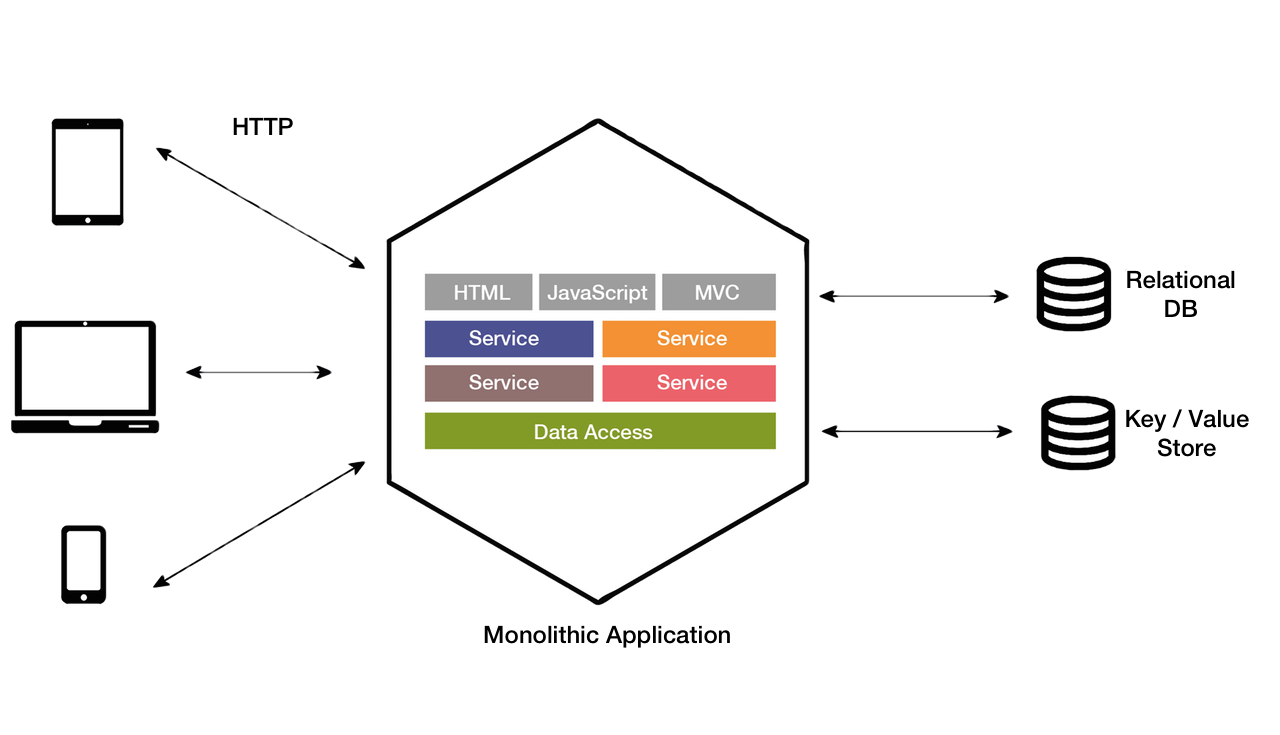
\includegraphics[width=\textwidth/2]{immagini/monolithic_architecture.png} % FONTE: https://medium.com
	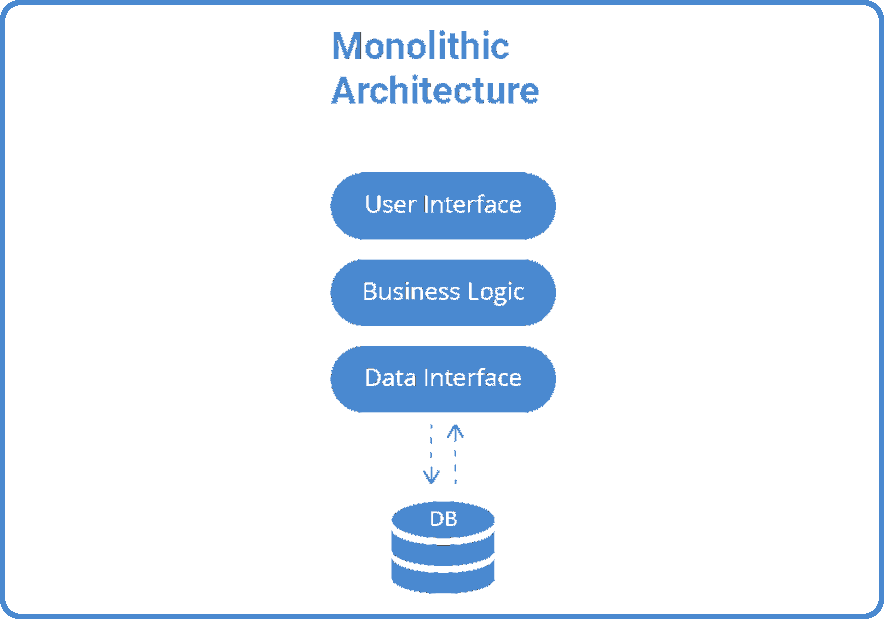
\includegraphics[width=\textwidth]{immagini/monolithic_architectureB.png} % FONTE: https://www.sam-solutions.com/blog/microservices-vs-monolithic-real-business-examples/
	\caption[Architettura monolitica]{Architettura monolitica}%\footnotemark}
	\label{fig:monolithic-arch}
\end{figure}
%\footnotetext{Fonte immagine: \href{https://www.sam-solutions.com/blog/microservices-vs-monolithic-real-business-examples/}{https://www.sam-solutions.com}}

Come è possibile notare dall'immagine, la \textit{business logic}, la gestione dei dati persistenti e la \gls{ui}, sono racchiusi in un unico grande monolite, termine da cui è stato tratto il nome di questa architettura.

Che tipo di vantaggi può comportare adottare tale architettura?

% https://microservices.io/patterns/monolithic.html

\paragraph*{Sviluppo} Sviluppare un'applicazione monolitica è per natura semplice, poiché tutto ciò che serve è racchiuso in un unico, talvolta grande, progetto, e gli strumenti di sviluppo e/o gli \gls{ide} 
hanno un ottimo supporto in tale contesto.

\paragraph*{Deploy} Fare un \gls{deploy}\gloss\ dell'applicativo, ossia un rilascio, è banale e diretto, poiché è sufficiente ricompilare il progetto (se previsto dallo \textit{stack} tecnologico utilizzato) e rilasciarlo nell'ambiente di produzione.

\paragraph*{Facile da scalare} Per far scalare l'applicazione, è sufficiente farne girare copie multiple contemporaneamente, con la possibilità di utilizzare un \textit{load balancer}.

\paragraph*{Testabilità} Facile da testare, poiché si ha il controllo di tutti gli \textit{input} e gli \textit{output}, con possibilità di \gls{mocking}\gloss\ dei \textit{layer}.

\bigskip
Veniamo ora agli svantaggi all'approccio monolitico.

\paragraph*{Dimensione intimidatoria} Al crescere delle dimensioni del progetto, diventa sempre più complicato individuare nuovi sviluppatori pronti ad apportare cambiamenti per nuove \textit{release},
viste le considerevoli dimensioni della \textit{code base}.
%Questo per via delle considerevoli dimensioni della \textit{code base}. che in applicazioni a livello \textit{enterprise} sono sempre di spessore non trascurabile.

\paragraph*{Continuous deployment} La pratica del \textit{continuous deployment} non è generalmente praticabile.
Per aggiornare un singolo componente, è necessario fare il ri-\gls{deploy} dell'intera applicazione, comportando minuti, se non ore, di totale indisponibilità del
servizio, nel suo complesso.
Per questo va effettuata una rigorosa pianificazione dei rilasci, nei periodi in cui l'applicativo viene usufruito di meno.

\paragraph*{Scalabilità} Mentre risulta facile scalare l'applicazione, lo stesso \textit{scaling} non è altrettanto efficacie. Tutti i dati risiedono in un unico, potenzialmente
enorme, \textit{persistence layer}. Quando la mole di dati inizia ad essere
consistente, ogni componente, per ottenere i dati, deve passare attraverso quest'unico \textit{layer}, che comporta un alto traffico di IO, oltre che un attesa dovuta all'attesa del recupero dei dati dall'eventuale \textit{database}.

\paragraph*{Stack tecnologico} L'inizio dello sviluppo di un applicativo monolitico richiede un ``contratto'' a lungo termine con una \textit{stack} tecnologico limitato. Una volta effettuata la scelta, non sarà possibile cambiare tecnologie per tutto il ciclo di vita del software (a meno che il prodotto non venga riscritto da zero), poiché tutte le componenti sono unite e dipendenti dalle tecnologie iniziali.

Gli svantaggi penalizzano molto fattori che riguardano la scalabilità
e progetti con target verso i \gls{big-data}.
Ecco perché negli ultimi anni il paradigma dei \glsdisp{microservizio}{microservizi} ha guadagnato
sempre più popolarità ed è sulla bocca di tutti.

\clearpage

% ------------------------------------------------------------------

\subsection{Architettura a microservizi}

Un'architettura a \glsdisp{microservizio}{microservizi} può essere genericamente vista come
nella figura\footcite{site:microservices-architecture} che segue:

\begin{figure}[H]
	\centering
	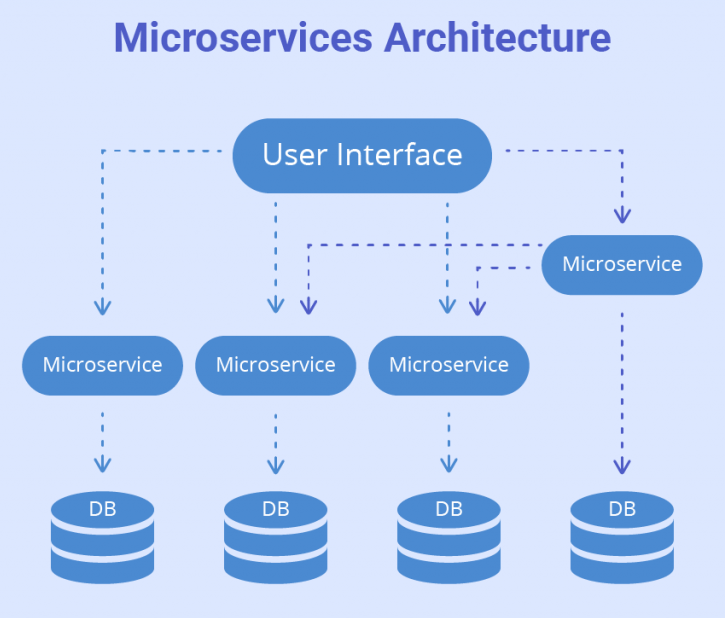
\includegraphics[width=\textwidth]{immagini/microservices_architecture.png} % FONTE: https://www.sam-solutions.com/blog/microservices-vs-monolithic-real-business-examples/
	\caption[Architettura a microservizi]{Architettura  a microservizi}
	\label{fig:microservices-arch}
\end{figure}
%\footnotetext{Fonte immagine: \href{https://www.sam-solutions.com/blog/microservices-vs-monolithic-real-business-examples/}{https://www.sam-solutions.com}}

Qui il sistema non è composto da un unico grande monolite, ma viene suddiviso in molti componenti indipendenti, chiamati \glsdisp{microservizio}{microservizi}, poiché contenuti e di limitata responsabilità.
È buona prassi dare a ognuno di essi una singola responsabilità, ove possibile, aderendo al \gls{srp}\gloss.

Come si può vedere in figura \ref{fig:microservices-arch}, ogni \gls{microservizio} ha un suo database da cui poter attingere.

Per poter comunicare, ognuno di essi espone delle \gls{api}, comunemente via \acrshort{http} e opzionalmente viene sfruttata una coda di messaggi (e.g. \textit{Apache Kafka}) per sfruttare i vantaggi dell'asincronicità.

\medskip

Vediamo i vantaggi più salienti di un approccio a microservizi per un sistema software.

\paragraph*{Basso accoppiamento} Uno dei primi vantaggi a cui viene naturale pensare in sistema a \glsdisp{microservizio}{microservizi} è che mantiene un basso accoppiamento. I servizi, comunicando via \gls{api} \acrshort{http}, sono tra loro totalmente disaccoppiati e indipendenti.

\paragraph*{Manutenzione} La manutenzione, vista la responsabilità e dimensione limitata dei servizi, è di facile approccio.
Non avendo a che fare con \textit{code base} intimorenti come nell'architettura monolitica, scovare e risolvere \textit{bug} richiede
molte meno risorse e tempo, poiché localizzati in un perimetro contenuto.

\paragraph*{Continuous Deployment} La pratica del \textit{continuous deployment} è praticabile con semplicità.
Ogni microservizio può essere rilasciato indipendemente dagli altri,
evitando così la necessità di dover programmare i rilasci che causano l'indisponibilità totale
dell'applicativo per tempo variabile.

\paragraph*{Divisione di business} Dividendo le responsabilità dei \glsdisp{microservizio}{microservizi}, è possibile dividere totalmente i compiti aziendali in base alle
competenze: chi si occupa di \textit{back-end}, potrà occuparsi esclusivamente di
\textit{back-end}, così come chi si occupa di \textit{front-end}, sviluppo di app per \textit{smartphone}, \gls{ui}/\acrshort{ux} \textit{Design} etc\dots

\paragraph*{Scalabilità} Uno dei maggiori punti di forza dei \glsdisp{microservizio}{microservizi} è l'alta scalabilità. La loro natura rende semplice scalare le
applicazioni: nessun servizio avrà una mole di dati enorme da gestire e risponderà in modo rapido. Aggiungendone di nuovi, gli esistenti non vengono rallentati, cosa che invece può accadere aggiungendo funzionalità in un monolite.

\bigskip

Ovviamente, la scelta di tale stile architetturale porta con sé diversi svantaggi che non vanno sottovalutati. Vediamone alcuni.

\paragraph*{Testabilità} Vista la natura distribuita dei \glsdisp{microservizio}{microservizi}, i \textit{test} di integrazione e di sistema possono risultare veramente complessi
da attuare. Ad esempio, alcuni servizi potrebbero essere momentaneamente non disponibili, altri con problemi non risolti, invalidando i \textit{test}.

\paragraph*{Complessità architetturale} I \glsdisp{microservizio}{microservizi} portano con sé complessità architetturale che in un monolite non è presente.
Con essa, sviluppatori e ingegneri devono tenere conto di molti più fattori, quali:
\begin{itemize}
	\item latenza della rete;
	\item \textit{fault tolerance}: capita spesso che un servizio non sia disponibile. Per questo va previsto un meccanismo di gestione delle
	condizioni di errore (\hyperref[circuit-breaker]{Circuit Breaker pattern});
	\item \textit{message parsing}: per la comunicazione molto spesso vengono usati messaggi in formato \acrshort{json}.
\end{itemize}

\paragraph*{Comunicazione} Per poter funzionare, i microservizi necessitano di meccanismi per poter comunicare e scambiare messaggi tra loro.

\subsection{Monolite vs. Microservizi: casi d'uso}
% TODO
Monolite

% ------------------------------------------------------------------

\section{Design pattern per microservizi}

Implementare un'architettura a \glsdisp{microservizio}{microservizi} non è una pratica semplice: non è sufficiente dividere il sistema in tanti componenti disaccoppiati per poter dire che un sistema segue questo paradigma.
Vanno seguite le \textit{best practice} delineate da chi si è trovato ad affrontare gli stessi problemi in precedenza.
Tra queste sono stati estrapolati nel corso degli anni diversi \gls{design-pattern}\gloss\ per poter raggiungere tale obiettivo.

Segue la discussione solo di alcuni di essi, quelli ritenuti di maggior interesse:

\begin{itemize}
	\item \textit{API Gateway};
	\item \textit{Aggregator};

	\item \textit{Database per service};
	\item \textit{Saga};

	\item \textit{Service discovery};
%	\item \textit{Log aggregation};
%	\item \textit{Health check};
	\item \textit{Circuit breaker}.
\end{itemize}

% ------------------------------------------------------------------

\subsection{API Gateway pattern}\label{api-gateway}

\paragraph*{Problema} Immaginiamo di avere un applicativo che  che debba supportare diversi tipi di interfaccia utente, quali: 
\begin{itemize}[noitemsep]
	\item una pagina web che utilizza le normali tecnologie del web, quali \acrshort{html} 5, \acrshort{css} e \gls{javascript};
	\item applicazione Android e iOS.
\end{itemize}

L'applicazione in questione potrebbe mettere a disposizione i seguenti servizi (sotto forma di microservizi):
\begin{itemize}[noitemsep]
	\item servizio informativo;
	\item servizio di login;
	\item servizio di registrazione;
	\item servizio di inventario;
	\item e così via.
\end{itemize}

\begin{figure}[H]
	\centering
	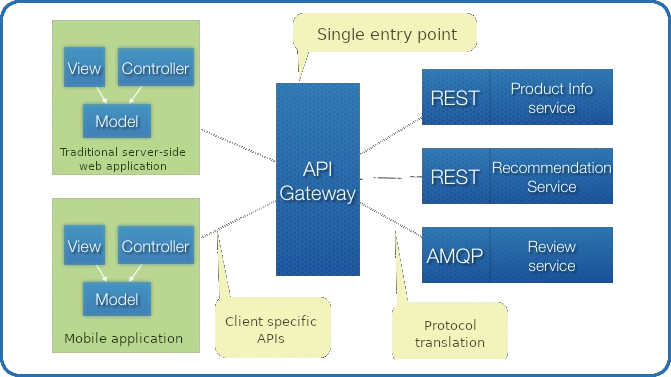
\includegraphics[width=\textwidth]{immagini/apigateway.png}
	\caption[Esempio d'uso API Gateway]{Esempio d'uso 'API Gateway pattern\footnotemark}
	\label{fig:api-gateway}
\end{figure}
\footnotetext{\cite{site:fonte-api-gateway}}

Come possono i vari consumatori dell'app sapere a quale \gls{microservizio} accedere per una determinata funzionalità?

\paragraph*{Soluzione} Mettere a disposizione un unico punto d'entrata per l'intero sistema, per tutti i \textit{client}.
Questo \textit{entry point} viene chiamato \textit{API Gateway}.

Esso gestisce le richieste principalmente in due modi:
mappandole verso i servizi che si occupano di quel compito specifico oppure espandendo la singola richiesta a multiple chiamate di vari servizi distinti.

Ci sono almeno un paio di varianti dell'\textit{API Gateway}:

\begin{itemize}
	\item esporre \gls{api} diverse, differenziate per tipo di client;
	\item definire un \textit{API Gateway} differente per ogni tipo di client.
\end{itemize}

% ------------------------------------------------------------------

\subsection{Aggregator pattern}

\paragraph*{Problema} Quando si dividono le funzionalità del \textit{business} in tanti piccoli frammenti logici (i \glsdisp{microservizio}{microservizi}), è necessario pensare
a come far collaborare i dati ottenuti da ognuno di essi.
Questa non è una responsabilità che può essere lasciata ai consumatori del servizio, anche perché li potrebbe portare a comprendere l'implementazione interna del prodotto, rompendo il principio di \gls{information-hiding}\gloss.

\paragraph*{Soluzione} L'\textit{Aggregator pattern} si occupa di risolvere questo problema: ``aggrega'' i dati ottenuti dai vari servizi e
manda la risposta finale ai consumatori.

Ci sono due modi di fare ciò:
\begin{itemize}
	\item un \gls{microservizio} composto che fa le chiamate ai servizi necessari
	unificando e trasformando i dati;
	\item Come detto in precedenza, un \textit{API Gateway} stesso può occuparsi di coprire il ruolo di \textit{aggregator}.
\end{itemize}

% ------------------------------------------------------------------

\subsection{Database per service pattern}

\paragraph*{Problema} Ci sono alcuni concetti da tenere in considerazione quando si va a progettare un sistema a \glsdisp{microservizio}{microservizi}:
\begin{itemize}[noitemsep]
	\item i servizi vanno tenuti scarsamente accoppiati;
	\item alcune transazioni hanno bisogno di ottenere dati presenti in diversi servizi;
	\item i database hanno bisogno di essere replicati per poter scalare.
\end{itemize}

\paragraph*{Soluzione} Per risolvere i problemi sopra descritti, in fase di progettazione va previsto il paradigma di \textit{database per service}.
I dati persistenti di un servizio non possono essere acceduti direttamente da altri servizi, ma vanno ottenuti tramite le \gls{api} esposte dal servizio.

% ------------------------------------------------------------------

\subsection{Saga pattern}

\paragraph*{Problema} Immaginiamo di aver applicato il pattern ``database per service''.
A questo punto, i servizi sono scarsamente accoppiati, tuttavia sorge un nuovo problema: alcune funzionalità di \textit{business}, si diffondono su più servizi e serve un meccanismo per garantire la consistenza dei dati
tra i vari servizi. 

Come è possibile mantenere tale consistenza di dati?

\paragraph*{Soluzione} Implementare ogni transazione di \textit{business} come un saga in modo che, qualvolta avvenga una transazione, il saga pubblichi un messaggio o evento che inneschi il prossimo saga nella catena ad effettuare la propria transazione locale, che a sua volta pubblicherà il messaggio di transazione avvenuta.
Dev'essere previsto un meccanismo di \textit{rollback} di tutte le transazioni avvenute se una di esse nella catena fallisce, nel caso qualche regola venisse violata.

Ci sono due modi per coordinare il \textit{Saga pattern}:
\begin{itemize}
	\item \textit{Choreography}: ogni transazione locale pubblica un evento che scatena le transazioni locali in altri servizi;
	\item \textit{Orchestration}: un \textit{orchestrator} dice ai partecipanti quali transazioni locali eseguire.
\end{itemize}

\begin{figure}[H]
	\centering
	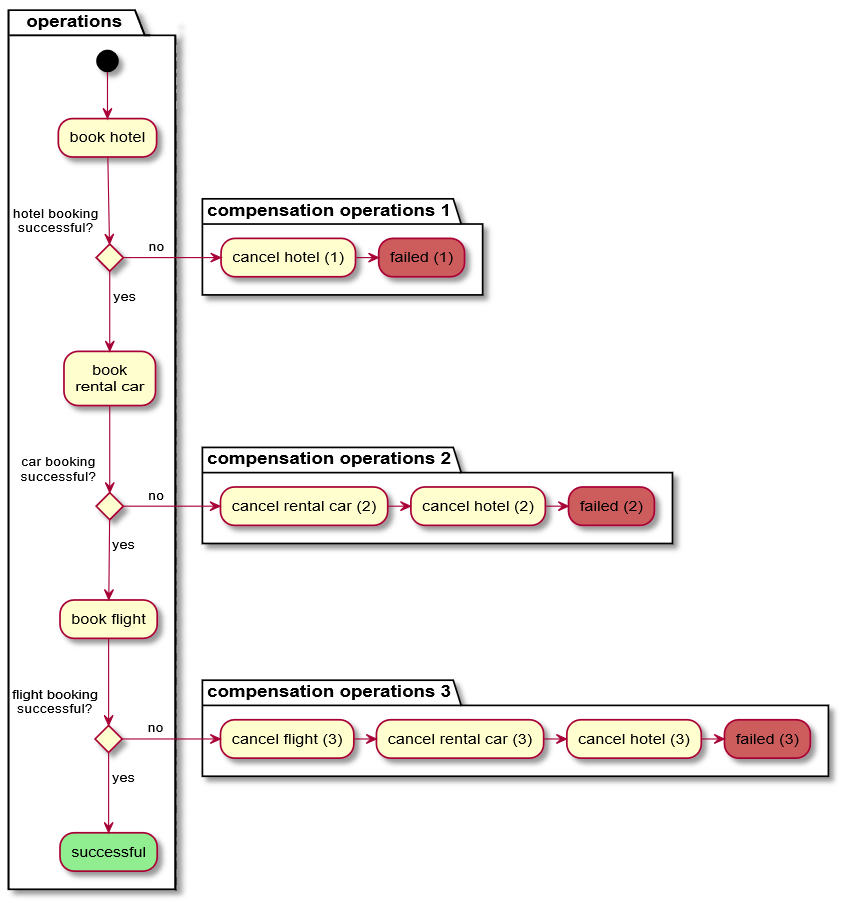
\includegraphics[width=0.8\textwidth]{immagini/saga-example.png}
	\caption[Esempio di Saga pattern]{Esempio di applicazione del Saga pattern\footnotemark}
\end{figure}
\footnotetext{\cite{site:fonte-saga}}

% ------------------------------------------------------------------

\subsection{Service Discovery pattern}\label{service-discovery}

\paragraph*{Problema} In un'architettura basata su \glsdisp{microservizio}{microservizi}, come si può gestire il \textit{routing}, ossia il processo di selezione di un percorso su una rete, che sarà comunemente composta da diverse istanze di più servizi?
Ogni servizio avrà il suo indirizzo (mappato su una porta specifica):  in un sistema distribuito non è ragionevole tenere traccia degli indirizzi manualmente, poiché l'IP di \gls{container}\gloss\ e \glsdisp{macchina-virtuale}{macchine virtuali}\gloss\ è spesso assegnato dinamicamente, cambiando nel tempo.

È necessario avere un processo che si occupi di tenere traccia di tutti i servizi coinvolti nel sistema e permetta di scoprire la loro posizione nella rete.

\paragraph*{Soluzione} Va fornito un \textit{Service Registry} che abbia esattamente questo ruolo:
ogni istanza di ogni servizio che viene inizializzata, registrata nel \textit{Service Registry}, mentre ogni istanza non disponibile o eliminata va rimossa dal registro.

\begin{figure}[H]
	\centering
	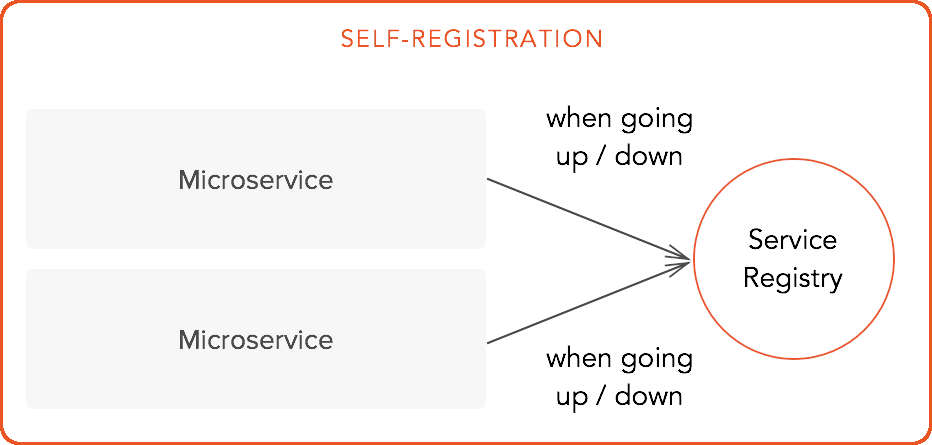
\includegraphics[width=\textwidth]{immagini/service-registry.png}
	\caption[Service Registry]{Service registry\footnotemark}
\end{figure}
\footnotetext{\cite{site:fonte-service-registry}}

L'attività di ``scoperta'' dei \glsdisp{microservizio}{microservizi} è chiamata \textit{Service Discovery}. Ne sono presenti due tipi:
\begin{itemize}
	\item \textit{Client-side discovery};
	\item \textit{Server-side discovery}.
\end{itemize}
Alcuni esempi saranno discussi in \S\ref{cap:spring-cloud}.

% ------------------------------------------------------------------

\subsection{Circuit Breaker pattern}\label{circuit-breaker}

\paragraph*{Problema} È comune in sistemi distribuiti fare chiamate remote a software che girano in processi differenti, probabilmente in macchine diverse di una rete.
La più grande differenza tra chiamate \textit{in-memory} e chiamate remote è che queste ultime possono fallire, o rimanere pendenti senza dare alcuna risposta finché il limite di tempo massimo viene raggiunto.

Questo può causare chiamate fallimentari a cascata che possono minare l'esperienza utente e rallentare il server. Come evitare il fallimento delle chiamate remote e gestire gli errori in modo robusto?

\begin{figure}[H]
	\centering
	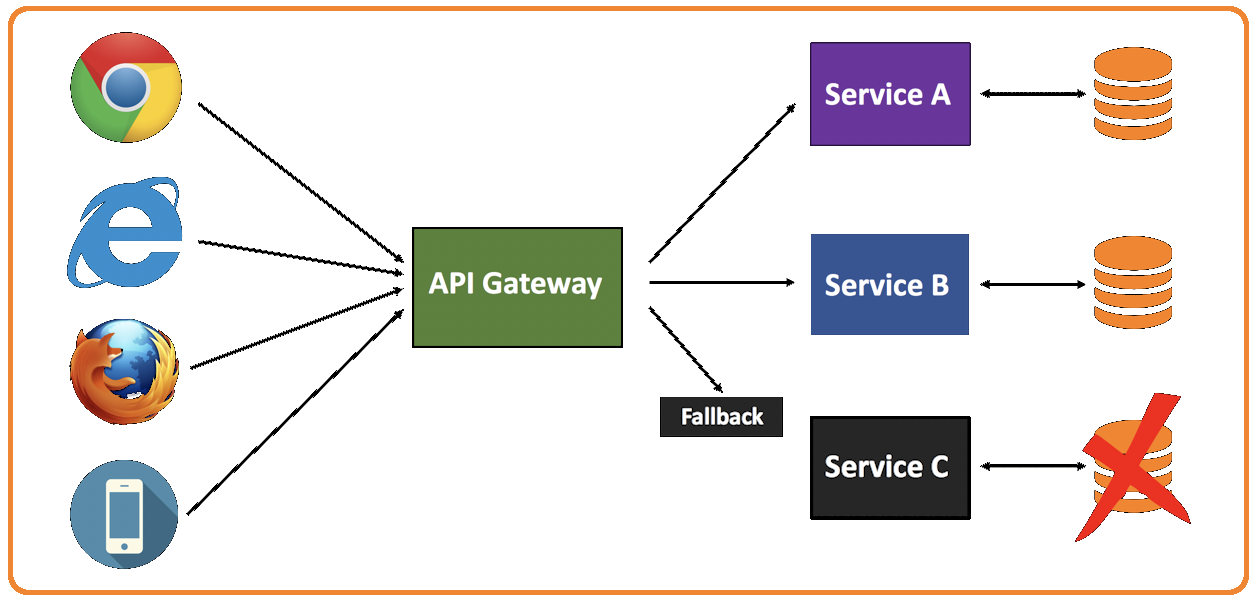
\includegraphics[width=\textwidth]{immagini/circuit-breaker.png}
	\caption[Esempio di Circuit Breaker]{Esempio di Circuit Breaker\footnotemark}
\end{figure}
\footnotetext{\cite{site:fonte-circuit-breaker}}

\paragraph*{Soluzione} Il \textit{client} dovrebbe chiamare i servizi remoti tramite un \textit{proxy} che si comporta come un interruttore di un circuito elettrico: quando il numero di chiamate fallite raggiunge una cerca soglia, l'interruttore viene azionato e per una durata di tempo specificata e configurabile tutte le chiamate remote al servizio falliranno immediatamente.

Passato il periodo di tempo, l'interruttore viene nuovamente disabilitato e le chiamate al servizio possono riprendere, eventualmente con un limite di carico per testare se il servizio effettivamente è tornato a funzionare a pieno regime.

% TODO Log aggregation

% TODO Health check

% TODO load balancer ?            % Appendice A
% !TEX encoding = UTF-8
% !TEX TS-program = pdflatex
% !TEX root = ../tesi.tex

%**************************************************************
\chapter{Spring Cloud}\label{cap:spring-cloud}
%**************************************************************

%\epigraph{Citazione}{Autore della citazione}

\intro{Spring Cloud è un \textit{framework} del team Pivotal che offre gli strumenti necessari agli sviluppatori per implementare alcuni dei \textit{pattern} più comuni per i sistemi distribuiti,
quali ad esempio \textit{Service Discovery}, \textit{Circuit Breaker} e \textit{Intelligent Routing} (\textit{API Gateway}).}

\bigskip

Coordinare sistemi distribuiti basati su microservizi porta notoriamente a cosiddetti \textit{boiler plate practices}. \textit{Spring Cloud} subentra offrendo dei meccanismi che implementano le pratiche comuni, per fornire robustezza e automazione nella gestione dei sistemi distribuiti.

\clearpage

%--------------------------------------------------------------------------------------

\section{Spring Cloud Config}

\textit{Spring Cloud Config} è il modulo con il compito di gestire le configurazioni del sistema distribuito: copre il ruolo di \textit{Configuration Management}.
Viene fornita la possibilità di configurare sia il \textit{client side} che il \textit{server side}.

\subsection{Configurazioni lato client} Le configurazioni \textit{client side} si effettuano tramite
il file \texttt{bootstrap.properties}. Ad esempio, per configurare il nome dell'applicazione, si deve
modificare la proprietà \texttt{spring.application.name}, aggiungendo al file sopracitato il rigo:

\begin{tcolorbox}
\texttt{spring.application.name: myapp}
\end{tcolorbox}\addcontentsline{codes}{section}{Cambio nome applicazione (Spring)}

Le configurazioni \texttt{bootstrap} sono mostrate all'\textit{endpoint} \texttt{/env}, come mostrato nell'esempio che segue, assumendo che il servizio sia locato all'indirizzo \texttt{http://localhost:8080}:

\begin{tcolorbox}
	\begin{verbatim}
		$ curl localhost:8080/env
		{
		"profiles":[],
		"configService:https://github.com/spring-samples/
		config-repo/bar.properties":{"foo":"bar"},
		"servletContextInitParams":{},
		"systemProperties":{...},
		...
		}
	\end{verbatim}
\end{tcolorbox}\addcontentsline{codes}{section}{Esempio Spring Cloud client side configuration}

\subsection{Configurazioni lato server} Per abilitare la configurazione lato server, va usata l'annotazione \texttt{@EnableConfigServer}, come nello \textit{snippet} che segue:

\begin{tcolorbox}
	\begin{lstlisting}
@SpringBootApplication
@EnableConfigServer
public class ConfigServer {
  public static void main(String[] args) {
    SpringApplication.run(ConfigServer.class, args);
  }
}
	\end{lstlisting}
\end{tcolorbox}\addcontentsline{codes}{section}{Attivazione server side configuration (Spring Cloud)}

La strategia che governa la configurazione lato server è \texttt{EnvironmentRepository}, che serve oggetti \texttt{Environment}.

Le risorse \texttt{Environment} sono parametrizzate da tre variabili:
\begin{itemize}
	\item \texttt{\{application\}}: mappa \texttt{spring.application.name} del lato client;
	\item \texttt{\{profile\}}: mappa \texttt{spring.profiles.active} del lato client, che indica il profilo attivo (sviluppo, produzione, etc\dots);
	\item \texttt{\{label\}}: etichetta un insieme di file di configurazione.
\end{itemize}

Come default, \texttt{EnvironmentRepository} usa come \textit{backend} il sistema di controllo versione \textit{Git}.
La proprietà \texttt{spring.cloud.config.server.git.uri} può essere impostata per cambiare l'URL della repository di \textit{back-end}.
Può puntare sia a una \textit{repository} remota (tramite prefissi \texttt{http:}, \texttt{https:}, etc\dots) che una locale (tramite il prefisso \texttt{file:}).

Tramite \textit{Cloud Config} è possibile fare una miriade di altre configurazioni, tra cui:

\begin{itemize}
	\item Disabilitare la validazione tramite certificato SSL;
	\item Impostare un \textit{timeout} per la connessione HTTP;
	\item Supportare multiple \textit{repository};
	\item Supportare l'autenticazione.
\end{itemize}

\subsection{Health indicator} \textit{Cloud Config} supporta nativamente un indicatore che
tiene sotto controllo lo stato dell'\texttt{Environment Repository} configurata.
È possibile disabilitare tale indicatore impostando la proprietà \texttt{spring.cloud.config.server.health.enabled} a falso.

\bigskip

\textit{Spring Cloud Config} offre molte altre opzioni e funzionalità che non verranno ulteriormente approfondite, poiché lo scopo di questa appendice è quello di dare una semplice infarinatura sul \textit{framework}.

%--------------------------------------------------------------------------------------

\section{Service Discovery con Netflix Eureka}

Per implementare il pattern \textit{Service Discovery} (discusso in \S\ref{service-discovery}) e molti altri, Spring si appoggia a \textit{Netflix Open Source Software} (\textit{Netflix OSS}), una raccolta di librerie offerte da Netflix.
Integra \textit{Netflix Eureka} come servizio con ruolo di \textit{Service Discovery}, lato client e server. \textit{Spring Cloud} offre diverse alternative per i vari pattern, tuttavia ne verranno discussi solo alcuni.

\begin{figure}[H]
	\centering
	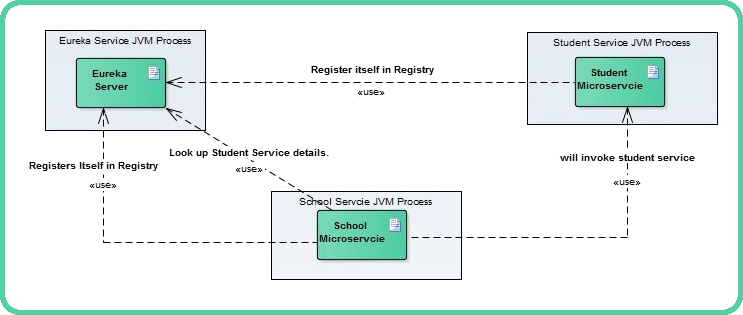
\includegraphics[width=\textwidth]{immagini/netflix-eureka.png}
	\caption[Spring Cloud Service Discovery con Netflix Eureka]{Spring Cloud Service Discovery con Netflix Eureka\footnotemark}
	\label{netflix-eureka}
\end{figure}
\footnotetext{Fonte immagine: \href{https://howtodoinjava.com/spring-cloud/spring-cloud-service-discovery-netflix-eureka/}{https://howtodoinjava.com}}

Vedendo \ref{netflix-eureka}, è possibile notare che ogni \textit{client} può registrarsi a \texttt{Eureka Server}, fornendo meta-dati di sé stesso, tra cui \textit{host}, porta, URL dell'\textit{Health Indicator}, \textit{home page}, e altri dettagli.

\subsection{Uso di EurekaClient} Una volta che un'applicazione è registrata nel \textit{Service Discovery} di \textit{Eureka}, è possibile utilizzare \texttt{EurekaClient} per scoprire i servizi che sono registrati, come mostrato nell'esempio seguente:

 \begin{tcolorbox}
 	\begin{lstlisting}
@Autowired
private EurekaClient discoveryClient;

public String serviceUrl() {
  InstanceInfo instance = discoveryClient.getNextServerFromEureka("STORES", false);
  return instance.getHomePageUrl();
}
 	\end{lstlisting}
 \end{tcolorbox}\addcontentsline{codes}{section}{Discover dei servizi registrati su EurekaServer}

\texttt{@Autowired} è un'annotazione che permette di iniettare i cosiddetti \textit{bean} di \textit{Spring} tramite \textit{dependency injection}. Nella variabile \texttt{instance} saranno salvate le informazioni relative al servizio di interesse.

\subsection{EurekaServer} Per utilizzare un applicazione come \texttt{EurekaServer}, è sufficiente utilizzare l'annotazione \texttt{@EnableEurekaServer} nella classe contenente il \textit{main}.

%--------------------------------------------------------------------------------------

\section{Circuit Breaker con Netflix Hystrix}

\textit{Netflix} offre una libreria che implementa il \textit{Circuit Breaker pattern}, già discusso in \S\ref{circuit-breaker}: \textit{Hystrix}.

È possibile vedere l'interfaccia del servizio nella figura che segue:

\begin{figure}[H]
	\centering
	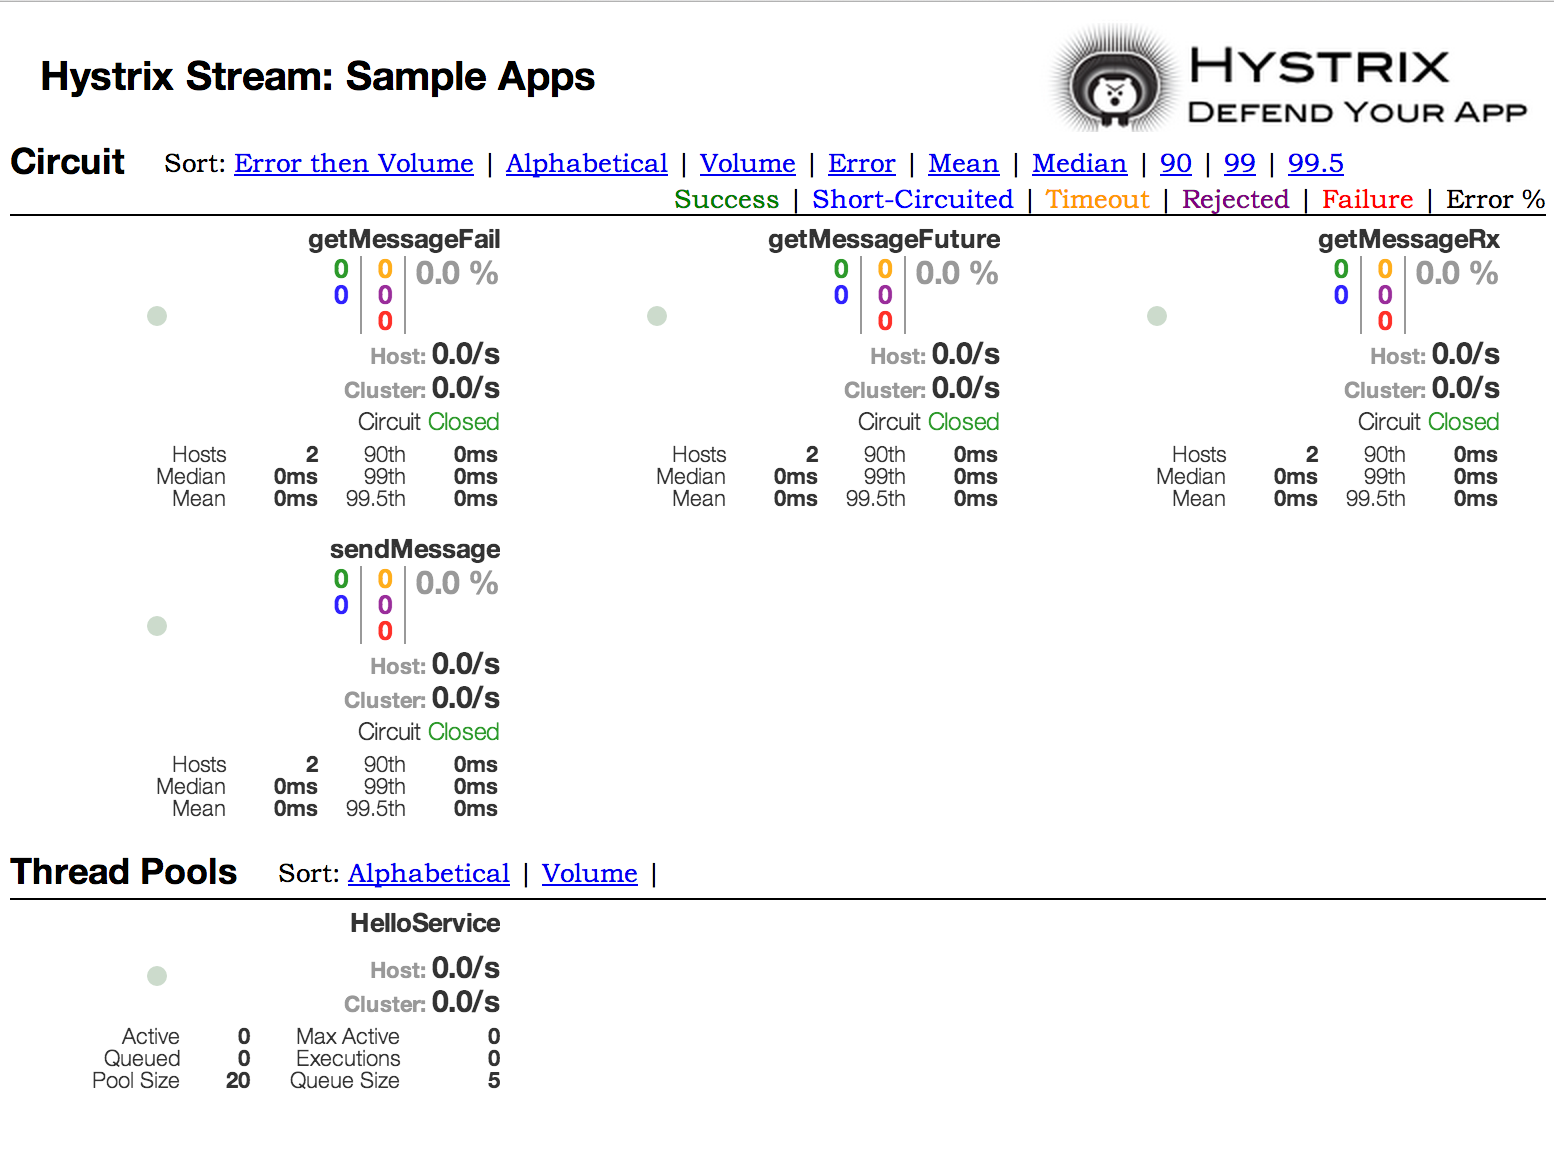
\includegraphics[width=\textwidth]{immagini/Hystrix.png}
	\caption[Interfaccia di Netflix Hystrix]{Interfaccia di Netflix Hystrix\footnotemark}
	\label{netflix-hystrix}
\end{figure}
\footnotetext{Fonte immagine: \href{https://cloud.spring.io/spring-cloud-static/Greenwich.SR1/single/spring-cloud.html}{https://cloud.spring.io}}

\textit{Spring Cloud} usa \textit{Hystrix} come \textit{Circuit Breaker}:
quando una chiamata a un particolare servizio eccede la proprietà \texttt{requestVolumeThreshold} (il valore di default è 20 richieste) e la percentuale di fallimento è maggiore di \texttt{errorThresholdPercentage} (default 50\%) in una finestra di tempo limitato,
il \textit{Circuit Breaker} si apre e le chiamate vengono prevenute e sostituite da chiamate di \textit{fallback} definite nel circuito.

\subsection{Abilitare Hystrix} Per abilitare \textit{Hystrix} in un'applicazione \textit{Spring},
è sufficiente usare l'annotazione \texttt{@EnableCircuitBreaker} nella classe contenente il \textit{main}.

Segue un minimale esempio d'uso di \textit{Hystrix}:


\begin{tcolorbox}
	\begin{lstlisting}
@Component
public class StoreIntegration {

  @HystrixCommand(fallbackMethod = "defaultStores")
  public Object getStores(Map<String, Object> parameters) {
    //do stuff that might fail
  }

  public Object defaultStores(Map<String, Object> parameters) {
    return /* something useful */;
  }
}
	\end{lstlisting}
\end{tcolorbox}\addcontentsline{codes}{section}{Esempio di Circuit Breaker con Netflix Hystrix}

Viene definito il metodo \texttt{getStores()} che effettua della logica con una \texttt{Map} passata come parametro.
L'annotazione \texttt{@HystrixCommand} definisce una chiamata di \textit{callback} in caso di attivazione del \textit{Circuit Breaker} verso il metodo \texttt{defaultStores()}.


%--------------------------------------------------------------------------------------

\section{API Gateway con Netflix Zuul}

Il \textit{routing} è una parte essenziale di un'architettura a microservizi. Come esempio, \texttt{/} potrebbe essere mappato sulla \textit{web application}, \texttt{/api/users} sul servizio utenti e \texttt{/api/shop} sul servizio di shopping.

\textit{Zuul} è un \textit{router} e \textit{load balancer} lato server basato su \textit{Java Virtual Machine} rilasciato da \textit{Netflix}. \textit{Spring Cloud} lo integra come \textit{router} principale. In quanto gestore del routing dei vari microservizi, svolge il ruolo di \textit{API Gateway} (discusso in \S\ref{api-gateway})

\begin{figure}[H]
	\centering
	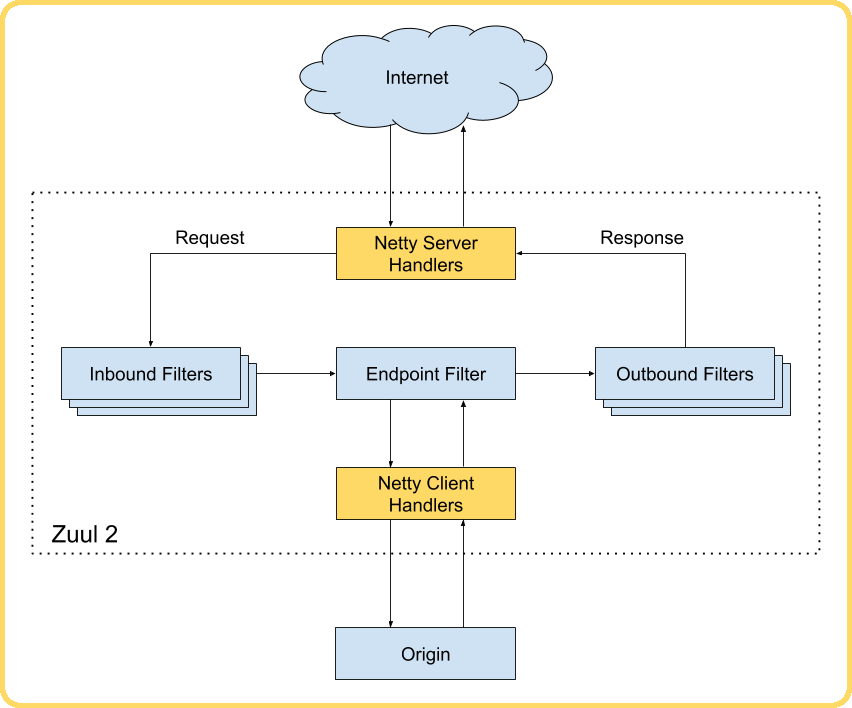
\includegraphics[width=\textwidth]{immagini/zuul.png}
	\caption[Panoramica di Netflix Zuul]{Panoramica di Netflix Zuul\footnotemark}
	\label{netflix-zuul}
\end{figure}
\footnotetext{Fonte immagine: \url{https://github.com/Netflix/zuul/wiki/How-It-Works-2.0}}

\subsection{Abilitare Zuul Reverse Proxy} Spring Cloud ha creato un \textit{proxy} integrato di \textit{Zuul} per aiutare lo sviluppo in casi d'uso comuni in cui un'applicazione UI voglia fare delle chiamate \textit{proxy} a uno o più servizi di \textit{back-end}, chiamato \textit{Zuul Reverse Proxy}.

Per abilitare \textit{Zuul Reverse Proxy}, basta annotare la classe \textit{main} con \texttt{@EnableZuulProxy}.

Sotto la proprietà \texttt{zuul.routes} sono elencati tutti i servizi gestiti dal \textit{routing} di \textit{Zuul}.
Vediamo un esempio.

\begin{tcolorbox}
	\begin{verbatim}
		zuul.routes.users.path: /myusers/**
	\end{verbatim}
\end{tcolorbox}\addcontentsline{codes}{section}{Configurazione di routing con Netflix Zuul}

In questo caso, tutte le chiamate a \texttt{/myusers} sono mappate all'\textit{endpoint} \texttt{/myusers} del servizio \texttt{users}.

È possibile ignorare alcuni pattern con la proprietà \texttt{zuul.ignoredPatterns}, per ragioni di sicurezza o altro, come ad esempio:

\begin{tcolorbox}
	\begin{verbatim}
	zuul.ignoredPatterns: /**/admin/**
	\end{verbatim}
\end{tcolorbox}\addcontentsline{codes}{section}{Pattern ignorati da Zuul}

In questo caso, considerando anche la proprietà impostata nell'esempio precedente, tutte le chiamate a \texttt{/myusers} vengono mappate tali quali a prima, ad eccezione di quelle che includono il \textit{pattern} \texttt{/admin/}, le quali vengono rigettate.

\subsection{Endpoint di Zuul} \textit{Zuul} mette a disposizione due \textit{endpoint}:
\begin{itemize}
	\item \texttt{/routes};
	\item \texttt{/filters}.
\end{itemize}

Una chiamata GET all'endpoint \texttt{/routes} può risultare in una risposta similare:

\begin{tcolorbox}
	\begin{verbatim}
{
    "/stores/**": "http://localhost:8081"
}
	\end{verbatim}
\end{tcolorbox}\addcontentsline{codes}{section}{Zuul: GET /routes}

Vengono restituiti tutti i servizi gestiti dal \textit{routing} di \textit{Zuul}, con nome e indirizzo originale.

Attraverso \texttt{/filters} è possibile ottenere una mappa dei filtri di \textit{Zuul} divisi per tipo.

%--------------------------------------------------------------------------------------

\section{Spring Cloud Stream}

\textit{Spring Cloud Stream} è un modulo di \textit{Spring Cloud} che permette di connettere l'applicazione a un \textit{message broker},
ossia un gestore di code di messaggi (quali \textit{Apache Kafka} o \textit{RabbitMQ}).

Il modulo può essere visto comunemente come la ``fusione'' tra \textit{Spring Boot} e \textit{Spring Integration}.

\begin{figure}[H]
	\centering
	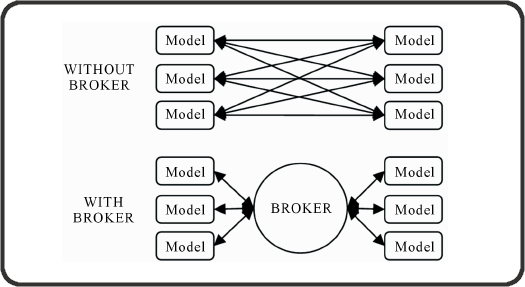
\includegraphics[width=0.8\textwidth]{immagini/message-broker.png}
	\caption[Message broker]{Message broker\footnotemark}
	\label{message-broker}
\end{figure}
\footnotetext{Fonte immagine: \url{https://www.researchgate.net}}

L'uso di un \textit{broker} permette di rendere i microservizi tra loro asincroni e trasferire alcune responsabilità di \textit{business logic} alla gestione dei messaggi del \textit{broker} stesso.

Comunicando esclusivamente via HTTP non si avrebbe il vantaggio dell'asincronicità dei microservizi: cosa succederebbe se il \textit{client} A notificasse un evento di interesse del \textit{client} B, immaginando che quest'ultimo sia momentaneamente indisponibile?
In caso di servizi sincroni, il messaggio verrebbe perso. Avendo invece a disposizione una coda di messaggi, il \textit{client} B potrebbe recuperare il messaggio in qualsiasi momento, una volta tornato disponibile.

Vediamo un esempio d'uso di \textit{Spring Cloud Stream}.
\begin{tcolorbox}
	\begin{lstlisting}
@SpringBootApplication
@EnableBinding(Sink.class)
public class LoggingConsumerApplication {

  public static void main(String[] args) {
    SpringApplication.run(LoggingConsumerApplication.class, args);
  }

  @StreamListener(Sink.INPUT)
  public void handle(Person person) {
    System.out.println("Received: " + person);
  }
}
	\end{lstlisting}
\end{tcolorbox}\addcontentsline{codes}{section}{Uso di Spring Cloud Stream}

Abbiamo il metodo \texttt{handle()} che gestisce i messaggi in entrata per il tipo \texttt{Person}.
Qui entra in gioco il \textit{framework}: cerca di convertire automaticamente il messaggio (in formato JSON) nel tipo \texttt{Person} riconosciuto dall'applicazione, che potrà usarlo per qualsivoglia logica.

In questo caso, stampa semplicemente a video un messaggio che mostra la persona ricevuta e convertita dal messaggio.

\bigskip

\textit{Spring Cloud Stream} offre dei \textit{binder} sia per \textit{Apache Kafka} che per \textit{Rabbit MQ}.

%**************************************************************
% Materiale finale
%**************************************************************

\backmatter
% !TEX encoding = UTF-8
% !TEX TS-program = pdflatex
% !TEX root = ../tesi.tex

%**************************************************************
% Bibliografia
%**************************************************************

\cleardoublepage
\chapter{Bibliografia}

%\nocite{*}
% Stampa i riferimenti bibliografici
%\printbibliography[heading=subbibliography,title={Riferimenti bibliografici},type=book]

% Stampa i siti web consultati
\printbibliography[heading=subbibliography,title={Siti web consultati},type=online]


\glsaddall
\printglossaries
\end{document}
